
% Default to the notebook output style

    


% Inherit from the specified cell style.




    
\documentclass[11pt]{article}

    
    
    \usepackage[T1]{fontenc}
    % Nicer default font (+ math font) than Computer Modern for most use cases
    \usepackage{mathpazo}

    % Basic figure setup, for now with no caption control since it's done
    % automatically by Pandoc (which extracts ![](path) syntax from Markdown).
    \usepackage{graphicx}
    % We will generate all images so they have a width \maxwidth. This means
    % that they will get their normal width if they fit onto the page, but
    % are scaled down if they would overflow the margins.
    \makeatletter
    \def\maxwidth{\ifdim\Gin@nat@width>\linewidth\linewidth
    \else\Gin@nat@width\fi}
    \makeatother
    \let\Oldincludegraphics\includegraphics
    % Set max figure width to be 80% of text width, for now hardcoded.
    \renewcommand{\includegraphics}[1]{\Oldincludegraphics[width=.8\maxwidth]{#1}}
    % Ensure that by default, figures have no caption (until we provide a
    % proper Figure object with a Caption API and a way to capture that
    % in the conversion process - todo).
    \usepackage{caption}
    \DeclareCaptionLabelFormat{nolabel}{}
    \captionsetup{labelformat=nolabel}

    \usepackage{adjustbox} % Used to constrain images to a maximum size 
    \usepackage{xcolor} % Allow colors to be defined
    \usepackage{enumerate} % Needed for markdown enumerations to work
    \usepackage{geometry} % Used to adjust the document margins
    \usepackage{amsmath} % Equations
    \usepackage{amssymb} % Equations
    \usepackage{textcomp} % defines textquotesingle
    % Hack from http://tex.stackexchange.com/a/47451/13684:
    \AtBeginDocument{%
        \def\PYZsq{\textquotesingle}% Upright quotes in Pygmentized code
    }
    \usepackage{upquote} % Upright quotes for verbatim code
    \usepackage{eurosym} % defines \euro
    \usepackage[mathletters]{ucs} % Extended unicode (utf-8) support
    \usepackage[utf8x]{inputenc} % Allow utf-8 characters in the tex document
    \usepackage{fancyvrb} % verbatim replacement that allows latex
    \usepackage{grffile} % extends the file name processing of package graphics 
                         % to support a larger range 
    % The hyperref package gives us a pdf with properly built
    % internal navigation ('pdf bookmarks' for the table of contents,
    % internal cross-reference links, web links for URLs, etc.)
    \usepackage{hyperref}
    \usepackage{longtable} % longtable support required by pandoc >1.10
    \usepackage{booktabs}  % table support for pandoc > 1.12.2
    \usepackage[inline]{enumitem} % IRkernel/repr support (it uses the enumerate* environment)
    \usepackage[normalem]{ulem} % ulem is needed to support strikethroughs (\sout)
                                % normalem makes italics be italics, not underlines
    

    
    
    % Colors for the hyperref package
    \definecolor{urlcolor}{rgb}{0,.145,.698}
    \definecolor{linkcolor}{rgb}{.71,0.21,0.01}
    \definecolor{citecolor}{rgb}{.12,.54,.11}

    % ANSI colors
    \definecolor{ansi-black}{HTML}{3E424D}
    \definecolor{ansi-black-intense}{HTML}{282C36}
    \definecolor{ansi-red}{HTML}{E75C58}
    \definecolor{ansi-red-intense}{HTML}{B22B31}
    \definecolor{ansi-green}{HTML}{00A250}
    \definecolor{ansi-green-intense}{HTML}{007427}
    \definecolor{ansi-yellow}{HTML}{DDB62B}
    \definecolor{ansi-yellow-intense}{HTML}{B27D12}
    \definecolor{ansi-blue}{HTML}{208FFB}
    \definecolor{ansi-blue-intense}{HTML}{0065CA}
    \definecolor{ansi-magenta}{HTML}{D160C4}
    \definecolor{ansi-magenta-intense}{HTML}{A03196}
    \definecolor{ansi-cyan}{HTML}{60C6C8}
    \definecolor{ansi-cyan-intense}{HTML}{258F8F}
    \definecolor{ansi-white}{HTML}{C5C1B4}
    \definecolor{ansi-white-intense}{HTML}{A1A6B2}

    % commands and environments needed by pandoc snippets
    % extracted from the output of `pandoc -s`
    \providecommand{\tightlist}{%
      \setlength{\itemsep}{0pt}\setlength{\parskip}{0pt}}
    \DefineVerbatimEnvironment{Highlighting}{Verbatim}{commandchars=\\\{\}}
    % Add ',fontsize=\small' for more characters per line
    \newenvironment{Shaded}{}{}
    \newcommand{\KeywordTok}[1]{\textcolor[rgb]{0.00,0.44,0.13}{\textbf{{#1}}}}
    \newcommand{\DataTypeTok}[1]{\textcolor[rgb]{0.56,0.13,0.00}{{#1}}}
    \newcommand{\DecValTok}[1]{\textcolor[rgb]{0.25,0.63,0.44}{{#1}}}
    \newcommand{\BaseNTok}[1]{\textcolor[rgb]{0.25,0.63,0.44}{{#1}}}
    \newcommand{\FloatTok}[1]{\textcolor[rgb]{0.25,0.63,0.44}{{#1}}}
    \newcommand{\CharTok}[1]{\textcolor[rgb]{0.25,0.44,0.63}{{#1}}}
    \newcommand{\StringTok}[1]{\textcolor[rgb]{0.25,0.44,0.63}{{#1}}}
    \newcommand{\CommentTok}[1]{\textcolor[rgb]{0.38,0.63,0.69}{\textit{{#1}}}}
    \newcommand{\OtherTok}[1]{\textcolor[rgb]{0.00,0.44,0.13}{{#1}}}
    \newcommand{\AlertTok}[1]{\textcolor[rgb]{1.00,0.00,0.00}{\textbf{{#1}}}}
    \newcommand{\FunctionTok}[1]{\textcolor[rgb]{0.02,0.16,0.49}{{#1}}}
    \newcommand{\RegionMarkerTok}[1]{{#1}}
    \newcommand{\ErrorTok}[1]{\textcolor[rgb]{1.00,0.00,0.00}{\textbf{{#1}}}}
    \newcommand{\NormalTok}[1]{{#1}}
    
    % Additional commands for more recent versions of Pandoc
    \newcommand{\ConstantTok}[1]{\textcolor[rgb]{0.53,0.00,0.00}{{#1}}}
    \newcommand{\SpecialCharTok}[1]{\textcolor[rgb]{0.25,0.44,0.63}{{#1}}}
    \newcommand{\VerbatimStringTok}[1]{\textcolor[rgb]{0.25,0.44,0.63}{{#1}}}
    \newcommand{\SpecialStringTok}[1]{\textcolor[rgb]{0.73,0.40,0.53}{{#1}}}
    \newcommand{\ImportTok}[1]{{#1}}
    \newcommand{\DocumentationTok}[1]{\textcolor[rgb]{0.73,0.13,0.13}{\textit{{#1}}}}
    \newcommand{\AnnotationTok}[1]{\textcolor[rgb]{0.38,0.63,0.69}{\textbf{\textit{{#1}}}}}
    \newcommand{\CommentVarTok}[1]{\textcolor[rgb]{0.38,0.63,0.69}{\textbf{\textit{{#1}}}}}
    \newcommand{\VariableTok}[1]{\textcolor[rgb]{0.10,0.09,0.49}{{#1}}}
    \newcommand{\ControlFlowTok}[1]{\textcolor[rgb]{0.00,0.44,0.13}{\textbf{{#1}}}}
    \newcommand{\OperatorTok}[1]{\textcolor[rgb]{0.40,0.40,0.40}{{#1}}}
    \newcommand{\BuiltInTok}[1]{{#1}}
    \newcommand{\ExtensionTok}[1]{{#1}}
    \newcommand{\PreprocessorTok}[1]{\textcolor[rgb]{0.74,0.48,0.00}{{#1}}}
    \newcommand{\AttributeTok}[1]{\textcolor[rgb]{0.49,0.56,0.16}{{#1}}}
    \newcommand{\InformationTok}[1]{\textcolor[rgb]{0.38,0.63,0.69}{\textbf{\textit{{#1}}}}}
    \newcommand{\WarningTok}[1]{\textcolor[rgb]{0.38,0.63,0.69}{\textbf{\textit{{#1}}}}}
    
    
    % Define a nice break command that doesn't care if a line doesn't already
    % exist.
    \def\br{\hspace*{\fill} \\* }
    % Math Jax compatability definitions
    \def\gt{>}
    \def\lt{<}
    % Document parameters
    \title{Operativsystemer og Netv?rk}
    
    
    

    % Pygments definitions
    
\makeatletter
\def\PY@reset{\let\PY@it=\relax \let\PY@bf=\relax%
    \let\PY@ul=\relax \let\PY@tc=\relax%
    \let\PY@bc=\relax \let\PY@ff=\relax}
\def\PY@tok#1{\csname PY@tok@#1\endcsname}
\def\PY@toks#1+{\ifx\relax#1\empty\else%
    \PY@tok{#1}\expandafter\PY@toks\fi}
\def\PY@do#1{\PY@bc{\PY@tc{\PY@ul{%
    \PY@it{\PY@bf{\PY@ff{#1}}}}}}}
\def\PY#1#2{\PY@reset\PY@toks#1+\relax+\PY@do{#2}}

\expandafter\def\csname PY@tok@w\endcsname{\def\PY@tc##1{\textcolor[rgb]{0.73,0.73,0.73}{##1}}}
\expandafter\def\csname PY@tok@c\endcsname{\let\PY@it=\textit\def\PY@tc##1{\textcolor[rgb]{0.25,0.50,0.50}{##1}}}
\expandafter\def\csname PY@tok@cp\endcsname{\def\PY@tc##1{\textcolor[rgb]{0.74,0.48,0.00}{##1}}}
\expandafter\def\csname PY@tok@k\endcsname{\let\PY@bf=\textbf\def\PY@tc##1{\textcolor[rgb]{0.00,0.50,0.00}{##1}}}
\expandafter\def\csname PY@tok@kp\endcsname{\def\PY@tc##1{\textcolor[rgb]{0.00,0.50,0.00}{##1}}}
\expandafter\def\csname PY@tok@kt\endcsname{\def\PY@tc##1{\textcolor[rgb]{0.69,0.00,0.25}{##1}}}
\expandafter\def\csname PY@tok@o\endcsname{\def\PY@tc##1{\textcolor[rgb]{0.40,0.40,0.40}{##1}}}
\expandafter\def\csname PY@tok@ow\endcsname{\let\PY@bf=\textbf\def\PY@tc##1{\textcolor[rgb]{0.67,0.13,1.00}{##1}}}
\expandafter\def\csname PY@tok@nb\endcsname{\def\PY@tc##1{\textcolor[rgb]{0.00,0.50,0.00}{##1}}}
\expandafter\def\csname PY@tok@nf\endcsname{\def\PY@tc##1{\textcolor[rgb]{0.00,0.00,1.00}{##1}}}
\expandafter\def\csname PY@tok@nc\endcsname{\let\PY@bf=\textbf\def\PY@tc##1{\textcolor[rgb]{0.00,0.00,1.00}{##1}}}
\expandafter\def\csname PY@tok@nn\endcsname{\let\PY@bf=\textbf\def\PY@tc##1{\textcolor[rgb]{0.00,0.00,1.00}{##1}}}
\expandafter\def\csname PY@tok@ne\endcsname{\let\PY@bf=\textbf\def\PY@tc##1{\textcolor[rgb]{0.82,0.25,0.23}{##1}}}
\expandafter\def\csname PY@tok@nv\endcsname{\def\PY@tc##1{\textcolor[rgb]{0.10,0.09,0.49}{##1}}}
\expandafter\def\csname PY@tok@no\endcsname{\def\PY@tc##1{\textcolor[rgb]{0.53,0.00,0.00}{##1}}}
\expandafter\def\csname PY@tok@nl\endcsname{\def\PY@tc##1{\textcolor[rgb]{0.63,0.63,0.00}{##1}}}
\expandafter\def\csname PY@tok@ni\endcsname{\let\PY@bf=\textbf\def\PY@tc##1{\textcolor[rgb]{0.60,0.60,0.60}{##1}}}
\expandafter\def\csname PY@tok@na\endcsname{\def\PY@tc##1{\textcolor[rgb]{0.49,0.56,0.16}{##1}}}
\expandafter\def\csname PY@tok@nt\endcsname{\let\PY@bf=\textbf\def\PY@tc##1{\textcolor[rgb]{0.00,0.50,0.00}{##1}}}
\expandafter\def\csname PY@tok@nd\endcsname{\def\PY@tc##1{\textcolor[rgb]{0.67,0.13,1.00}{##1}}}
\expandafter\def\csname PY@tok@s\endcsname{\def\PY@tc##1{\textcolor[rgb]{0.73,0.13,0.13}{##1}}}
\expandafter\def\csname PY@tok@sd\endcsname{\let\PY@it=\textit\def\PY@tc##1{\textcolor[rgb]{0.73,0.13,0.13}{##1}}}
\expandafter\def\csname PY@tok@si\endcsname{\let\PY@bf=\textbf\def\PY@tc##1{\textcolor[rgb]{0.73,0.40,0.53}{##1}}}
\expandafter\def\csname PY@tok@se\endcsname{\let\PY@bf=\textbf\def\PY@tc##1{\textcolor[rgb]{0.73,0.40,0.13}{##1}}}
\expandafter\def\csname PY@tok@sr\endcsname{\def\PY@tc##1{\textcolor[rgb]{0.73,0.40,0.53}{##1}}}
\expandafter\def\csname PY@tok@ss\endcsname{\def\PY@tc##1{\textcolor[rgb]{0.10,0.09,0.49}{##1}}}
\expandafter\def\csname PY@tok@sx\endcsname{\def\PY@tc##1{\textcolor[rgb]{0.00,0.50,0.00}{##1}}}
\expandafter\def\csname PY@tok@m\endcsname{\def\PY@tc##1{\textcolor[rgb]{0.40,0.40,0.40}{##1}}}
\expandafter\def\csname PY@tok@gh\endcsname{\let\PY@bf=\textbf\def\PY@tc##1{\textcolor[rgb]{0.00,0.00,0.50}{##1}}}
\expandafter\def\csname PY@tok@gu\endcsname{\let\PY@bf=\textbf\def\PY@tc##1{\textcolor[rgb]{0.50,0.00,0.50}{##1}}}
\expandafter\def\csname PY@tok@gd\endcsname{\def\PY@tc##1{\textcolor[rgb]{0.63,0.00,0.00}{##1}}}
\expandafter\def\csname PY@tok@gi\endcsname{\def\PY@tc##1{\textcolor[rgb]{0.00,0.63,0.00}{##1}}}
\expandafter\def\csname PY@tok@gr\endcsname{\def\PY@tc##1{\textcolor[rgb]{1.00,0.00,0.00}{##1}}}
\expandafter\def\csname PY@tok@ge\endcsname{\let\PY@it=\textit}
\expandafter\def\csname PY@tok@gs\endcsname{\let\PY@bf=\textbf}
\expandafter\def\csname PY@tok@gp\endcsname{\let\PY@bf=\textbf\def\PY@tc##1{\textcolor[rgb]{0.00,0.00,0.50}{##1}}}
\expandafter\def\csname PY@tok@go\endcsname{\def\PY@tc##1{\textcolor[rgb]{0.53,0.53,0.53}{##1}}}
\expandafter\def\csname PY@tok@gt\endcsname{\def\PY@tc##1{\textcolor[rgb]{0.00,0.27,0.87}{##1}}}
\expandafter\def\csname PY@tok@err\endcsname{\def\PY@bc##1{\setlength{\fboxsep}{0pt}\fcolorbox[rgb]{1.00,0.00,0.00}{1,1,1}{\strut ##1}}}
\expandafter\def\csname PY@tok@kc\endcsname{\let\PY@bf=\textbf\def\PY@tc##1{\textcolor[rgb]{0.00,0.50,0.00}{##1}}}
\expandafter\def\csname PY@tok@kd\endcsname{\let\PY@bf=\textbf\def\PY@tc##1{\textcolor[rgb]{0.00,0.50,0.00}{##1}}}
\expandafter\def\csname PY@tok@kn\endcsname{\let\PY@bf=\textbf\def\PY@tc##1{\textcolor[rgb]{0.00,0.50,0.00}{##1}}}
\expandafter\def\csname PY@tok@kr\endcsname{\let\PY@bf=\textbf\def\PY@tc##1{\textcolor[rgb]{0.00,0.50,0.00}{##1}}}
\expandafter\def\csname PY@tok@bp\endcsname{\def\PY@tc##1{\textcolor[rgb]{0.00,0.50,0.00}{##1}}}
\expandafter\def\csname PY@tok@fm\endcsname{\def\PY@tc##1{\textcolor[rgb]{0.00,0.00,1.00}{##1}}}
\expandafter\def\csname PY@tok@vc\endcsname{\def\PY@tc##1{\textcolor[rgb]{0.10,0.09,0.49}{##1}}}
\expandafter\def\csname PY@tok@vg\endcsname{\def\PY@tc##1{\textcolor[rgb]{0.10,0.09,0.49}{##1}}}
\expandafter\def\csname PY@tok@vi\endcsname{\def\PY@tc##1{\textcolor[rgb]{0.10,0.09,0.49}{##1}}}
\expandafter\def\csname PY@tok@vm\endcsname{\def\PY@tc##1{\textcolor[rgb]{0.10,0.09,0.49}{##1}}}
\expandafter\def\csname PY@tok@sa\endcsname{\def\PY@tc##1{\textcolor[rgb]{0.73,0.13,0.13}{##1}}}
\expandafter\def\csname PY@tok@sb\endcsname{\def\PY@tc##1{\textcolor[rgb]{0.73,0.13,0.13}{##1}}}
\expandafter\def\csname PY@tok@sc\endcsname{\def\PY@tc##1{\textcolor[rgb]{0.73,0.13,0.13}{##1}}}
\expandafter\def\csname PY@tok@dl\endcsname{\def\PY@tc##1{\textcolor[rgb]{0.73,0.13,0.13}{##1}}}
\expandafter\def\csname PY@tok@s2\endcsname{\def\PY@tc##1{\textcolor[rgb]{0.73,0.13,0.13}{##1}}}
\expandafter\def\csname PY@tok@sh\endcsname{\def\PY@tc##1{\textcolor[rgb]{0.73,0.13,0.13}{##1}}}
\expandafter\def\csname PY@tok@s1\endcsname{\def\PY@tc##1{\textcolor[rgb]{0.73,0.13,0.13}{##1}}}
\expandafter\def\csname PY@tok@mb\endcsname{\def\PY@tc##1{\textcolor[rgb]{0.40,0.40,0.40}{##1}}}
\expandafter\def\csname PY@tok@mf\endcsname{\def\PY@tc##1{\textcolor[rgb]{0.40,0.40,0.40}{##1}}}
\expandafter\def\csname PY@tok@mh\endcsname{\def\PY@tc##1{\textcolor[rgb]{0.40,0.40,0.40}{##1}}}
\expandafter\def\csname PY@tok@mi\endcsname{\def\PY@tc##1{\textcolor[rgb]{0.40,0.40,0.40}{##1}}}
\expandafter\def\csname PY@tok@il\endcsname{\def\PY@tc##1{\textcolor[rgb]{0.40,0.40,0.40}{##1}}}
\expandafter\def\csname PY@tok@mo\endcsname{\def\PY@tc##1{\textcolor[rgb]{0.40,0.40,0.40}{##1}}}
\expandafter\def\csname PY@tok@ch\endcsname{\let\PY@it=\textit\def\PY@tc##1{\textcolor[rgb]{0.25,0.50,0.50}{##1}}}
\expandafter\def\csname PY@tok@cm\endcsname{\let\PY@it=\textit\def\PY@tc##1{\textcolor[rgb]{0.25,0.50,0.50}{##1}}}
\expandafter\def\csname PY@tok@cpf\endcsname{\let\PY@it=\textit\def\PY@tc##1{\textcolor[rgb]{0.25,0.50,0.50}{##1}}}
\expandafter\def\csname PY@tok@c1\endcsname{\let\PY@it=\textit\def\PY@tc##1{\textcolor[rgb]{0.25,0.50,0.50}{##1}}}
\expandafter\def\csname PY@tok@cs\endcsname{\let\PY@it=\textit\def\PY@tc##1{\textcolor[rgb]{0.25,0.50,0.50}{##1}}}

\def\PYZbs{\char`\\}
\def\PYZus{\char`\_}
\def\PYZob{\char`\{}
\def\PYZcb{\char`\}}
\def\PYZca{\char`\^}
\def\PYZam{\char`\&}
\def\PYZlt{\char`\<}
\def\PYZgt{\char`\>}
\def\PYZsh{\char`\#}
\def\PYZpc{\char`\%}
\def\PYZdl{\char`\$}
\def\PYZhy{\char`\-}
\def\PYZsq{\char`\'}
\def\PYZdq{\char`\"}
\def\PYZti{\char`\~}
% for compatibility with earlier versions
\def\PYZat{@}
\def\PYZlb{[}
\def\PYZrb{]}
\makeatother


    % Exact colors from NB
    \definecolor{incolor}{rgb}{0.0, 0.0, 0.5}
    \definecolor{outcolor}{rgb}{0.545, 0.0, 0.0}



    
    % Prevent overflowing lines due to hard-to-break entities
    \sloppy 
    % Setup hyperref package
    \hypersetup{
      breaklinks=true,  % so long urls are correctly broken across lines
      colorlinks=true,
      urlcolor=urlcolor,
      linkcolor=linkcolor,
      citecolor=citecolor,
      }
    % Slightly bigger margins than the latex defaults
    
    \geometry{verbose,tmargin=1in,bmargin=1in,lmargin=1in,rmargin=1in}
    
    

    \begin{document}
    
    
    \maketitle
    
    

    
    \section{Generelt}\label{generelt}

\begin{itemize}
\tightlist
\item
  \textbf{Kontor} ADA-216
\end{itemize}

    \section{Virtual memory}\label{virtual-memory}

\begin{itemize}
\tightlist
\item
  An \textbf{operating system} from the programmers point of views adds
  a variety of new instructions beyond the ISA level

  \begin{itemize}
  \tightlist
  \item
    These instructions is called \textbf{system calls} which invokes a
    predefined operating system service, effectively, one of its
    instructions e.g. reading data from a file
  \item
    The Operating System Level (OSL) is always interpreted
  \end{itemize}
\item
  \textbf{Virtual memory} is a smart way to use memory which is not
  available

  \begin{itemize}
  \tightlist
  \item
    The words of memory and memory are separated so that 4096 words but
    they does not need to correspond to memory location 0 to 4096
    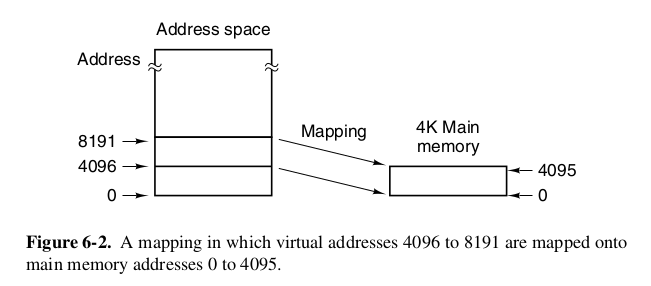
\includegraphics{img/memory_mapping.png}
  \item
    If the memory is mapped between 4096 to 8191 and the program
    branches to memory location between 8192 and 12287 and the machine
    has virtual memory the following happens (\textbf{paging})

    \begin{enumerate}
    \def\labelenumi{\arabic{enumi}.}
    \tightlist
    \item
      The contents of the main memory is saved on disk
    \item
      Words 8192 to 12287 would be located on disk.
    \item
      Words 8192 to 12287 would be loaded into main memory.
    \item
      The address map would be changed to map addresses 8192 to 12287
      onto memory locations 0 to 4095.
    \item
      Execution would continue as though nothing unusual had happened.
    \end{enumerate}
  \item
    The chunks of program read in from disk are called \textbf{pages}
  \item
    The addresses that a program refer to is called \textbf{virtual
    address space}
  \item
    The actual physical memory locations are called \textbf{physical
    address space}
  \item
    A \textbf{memory map} or \textbf{page table} specifies for each
    virtual address what the corresponding physical address is
  \item
    The paging mechanism is said to be \textbf{transparent} because the
    programming does not need to know that it exists.
  \end{itemize}
\end{itemize}

    \subsection{Implementation}\label{implementation}

\begin{itemize}
\tightlist
\item
  The virtual disk space is broken up into a number of equal size pages

  \begin{itemize}
  \tightlist
  \item
    Page sizes range from 512 to 64 KB pr page
  \item
    The page size is always the power of two, for example \(2^k\), so
    that all addresses can be represented in \(k\) bits
  \item
    The physical address space is broken into pieces in a similar way as
    the virtual ones
  \item
    The pieces of main memory into which the pages goes are called
    \textbf{page frames}

    \begin{itemize}
    \tightlist
    \item
      Typically thousands exists
    \end{itemize}
  \end{itemize}
\item
  The device for doing virtual-to-physical mapping is called \textbf{MMU
  (Memory Management Unit).}

  \begin{itemize}
  \tightlist
  \item
    may be on the CPU chip or a seperate chip
  \item
    To see if an page-table entry is currently in memory the MMU checks
    the \textbf{present/absent bit} in the page table entry
  \end{itemize}
\item
  When a reference is made to an address on a page not present in main
  memory, it is called a \textbf{page fault}.

  \begin{itemize}
  \tightlist
  \item
    After it has occurred the operating system must

    \begin{itemize}
    \tightlist
    \item
      read the required page from disk
    \item
      enter its new physical memory location in the page table
    \item
      then repeat the instruction that caused the fault.
    \end{itemize}
  \item
    In \textbf{demand paging}, a page is brought into memory only when a
    request for it occurs, not in advance.
  \item
    The \textbf{locality principle} is that references tend to cluster
    on a small number of pages.
  \item
    The \textbf{working set} is a set at any given time consisting of
    all the pages used by the k most recent memory references
  \end{itemize}
\end{itemize}

    \subsection{Page-Replacement Policy}\label{page-replacement-policy}

\begin{itemize}
\tightlist
\item
  When fetching a page an algorithm needs to decide which page to be
  sent back to disk

  \begin{itemize}
  \tightlist
  \item
    The \textbf{LRU (Least Recently Used)} algorithm evicts the page
    least recently
  \item
    \textbf{FIFO (First-In First-Out)} removes the least recently loaded
    page
  \item
    A program that generates page faults frequently and continuously is
    said to be thrashing.
  \item
    Many operating systems has a bit which tells if the page has been
    written to since it was loaded
  \end{itemize}
\item
  The problem of wasted bytes when only some of the pages are full are
  called \textbf{internal fragmentation}
\end{itemize}

    \subsection{Segmentation}\label{segmentation}

\begin{itemize}
\tightlist
\item
  A straightforward solution to overflowing memory is to provide many
  completely independent address spaces, called \textbf{segments}.

  \begin{itemize}
  \tightlist
  \item
    Each segment consists of a linear sequence of addresses, from 0 to
    some maximum.
  \item
    The length of a stack segment may be increased and decrease when the
    stack changes
  \item
    Different segments can grow and shrink independently without
    affecting each other
  \item
    It is very rare that a segment is filled up because it is very large
  \item
    To specify a segment the program must supply a two-part address: a
    segment number, and an address within the segment.
    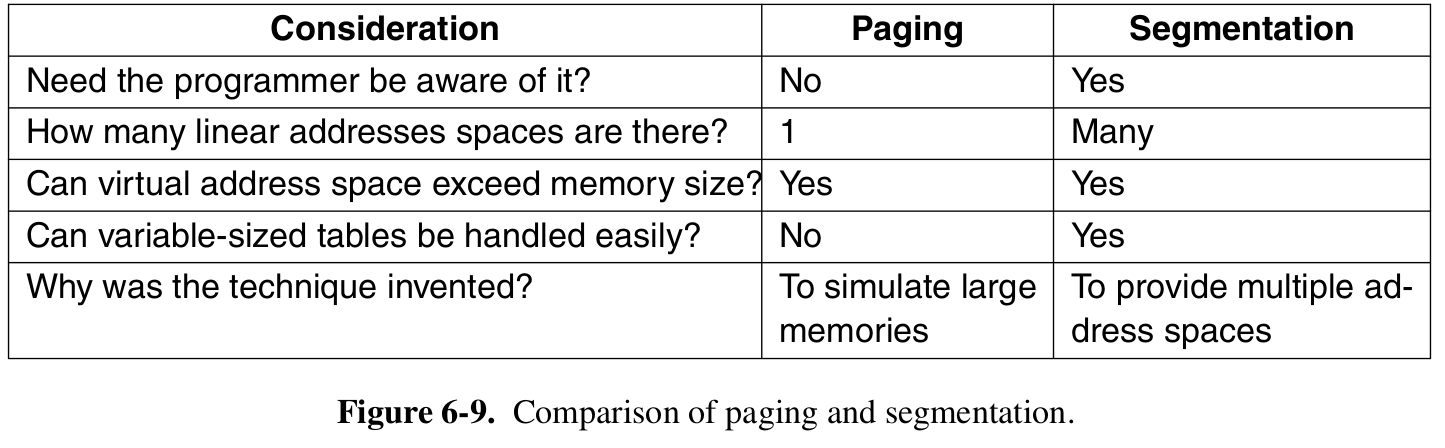
\includegraphics{img/paging_vs_segmentation.png}
  \end{itemize}
\item
  Segmentation can be implemented in one of two ways: swapping and
  paging

  \begin{itemize}
  \tightlist
  \item
    Segment swapping is not unlike demand paging: segment come and and
    segments go as needed

    \begin{itemize}
    \tightlist
    \item
      Implementation differs from paging because segments differs in
      size and paging does not
    \item
      \textbf{External fragmentation} is the phenomenon where after the
      computer has been running after some time the memory is containing
      segments and some containing holes
    \item
      \textbf{Compacting} is moving all the segments together to remove
      the external fragmentation
    \end{itemize}
  \item
    Paging is dividing each segment up into fixed-size pages and demand
    paging them.
  \end{itemize}
\end{itemize}

    \section{Threads}\label{threads}

\begin{itemize}
\item
  A \textbf{program} can contain multiple threads

  \begin{itemize}
  \tightlist
  \item
    Each thread has a lifetime extending from the first instruction
    executes to the last one
  \item
    If two threads has overlapping life time it is said that they are
    concurrent
  \end{itemize}
\item
  Command to compile C program with threads:
  \texttt{gcc\ -pthread\ program.c\ -o\ program.out}
\item
  Simple multi threaded program in C
\end{itemize}

\begin{Shaded}
\begin{Highlighting}[]
\PreprocessorTok{#include }\ImportTok{<pthread.h>}
\PreprocessorTok{#include }\ImportTok{<unistd.h>}
\PreprocessorTok{#include }\ImportTok{<stdio.h>}

\DataTypeTok{static} \DataTypeTok{void}\NormalTok{ * child(}\DataTypeTok{void}\NormalTok{ *ignored)\{}
\NormalTok{    sleep(}\DecValTok{3}\NormalTok{);}
\NormalTok{    printf(}\StringTok{"Child is done sleeping 3 seconds.}\SpecialCharTok{\textbackslash{}n}\StringTok{"}\NormalTok{);}
    \ControlFlowTok{return}\NormalTok{ NULL;}
\NormalTok{\}}
\DataTypeTok{int}\NormalTok{ main(}\DataTypeTok{int}\NormalTok{ argc, }\DataTypeTok{char}\NormalTok{ *argv[])\{}
\NormalTok{    pthread_t child_thread;}
    \DataTypeTok{int}\NormalTok{ code;}
\NormalTok{    code = pthread_create(&child_thread, NULL, child, NULL);}
    \ControlFlowTok{if}\NormalTok{(code)\{}
\NormalTok{        fprintf(stderr, }\StringTok{"pthread_create failed with code %d}\SpecialCharTok{\textbackslash{}n}\StringTok{"}\NormalTok{, code);}
\NormalTok{    \}}
\NormalTok{    sleep(}\DecValTok{5}\NormalTok{);}
\NormalTok{    printf(}\StringTok{"Parent is done sleeping 5 seconds.}\SpecialCharTok{\textbackslash{}n}\StringTok{"}\NormalTok{);}
    \ControlFlowTok{return} \DecValTok{0}\NormalTok{;}
\NormalTok{\}}
\end{Highlighting}
\end{Shaded}

    \subsection{Switching Between Threads}\label{switching-between-threads}

\begin{itemize}
\item
  To switch between different threads the processor needs to store
  information about that thread in memory

  \begin{itemize}
  \tightlist
  \item
    Saves the program counter, the contents of the registers and the
    stack pointer for higher order languages
  \item
    A block of memory containing information about a thread is called a
    \textbf{thread control block} or \textbf{task control block} (TCB)
  \end{itemize}
\item
  The registers can be pushed onto the stack before thread switching so
  thread switching is done as follows

\begin{verbatim}
push each register on the (outgoing thread’s) stack
store the stack pointer into outgoing->SP
load the stack pointer from next->SP
store label L’s address into outgoing->IP
load in next->IP and jump to that address
L:
pop each register from the (resumed outgoing thread’s) stack
\end{verbatim}
\item
  Thread switching is often called \textbf{context switching}
\end{itemize}

    \subsection{Preemptive Multitasking}\label{preemptive-multitasking}

\begin{itemize}
\tightlist
\item
  \textbf{Cooperative multitasking} is where each thread themselves
  contains explicit code at each point a thread switch should occur
\item
  \textbf{Preemptive multitasking} is where the threads code do not
  contain explicit code, where the thread switch should occur

  \begin{itemize}
  \tightlist
  \item
    It can still be useful for a thread to voluntarily give way to the
    other threads, normally called yield

    \begin{itemize}
    \tightlist
    \item
      The pthreads api uses\texttt{sched\_yield()}
    \end{itemize}
  \item
    The \texttt{ret} instruction used in the Linux code for thread
    switching.
  \end{itemize}
\item
  When an I/O device or timer needs attention an \textbf{interrupt}
  occurs and the processor jumps off to the special procedure called the
  \textbf{interrupt handler}

  \begin{itemize}
  \tightlist
  \item
    Is part of the operating system and deal with the hardware device
  \item
    When it is done it executes a return from interrupt instruction,
    which jumps back to the instruction which it interrupted
  \item
    It needs to handler needs to save all the registers at the start and
    restore them before returning.
  \item
    Can be used by an operating system to provide preemptive
    multitasking.

    \begin{itemize}
    \tightlist
    \item
      If the interrupt was from the timer and the current thread had
      been executing for a long time, it may be needed to switch to
      another thread
    \end{itemize}
  \end{itemize}
\end{itemize}

    \section{Scheduling}\label{scheduling}

\begin{itemize}
\tightlist
\item
  The \textbf{scheduler} chooses which thread to run at each time
\item
  Checking if an desired event has occurred is called \textbf{busy
  waiting}

  \begin{itemize}
  \tightlist
  \item
    Is a bad-idea
  \end{itemize}
\item
  The operating system keeps track of which threads are waiting and
  which can usefully run

  \begin{itemize}
  \tightlist
  \item
    The system does this by storing runnable threads in a \textbf{run
    queue} and the waiting in \textbf{waiting queues} one per reason for
    waiting

    \begin{itemize}
    \tightlist
    \item
      The threads which are waiting for a desired amount of time to
      elapse is stored in time order
    \end{itemize}
  \item
    The scheduler only considers threads in the run queue
  \item
    One of the services of the interrupt handler is do determine that a
    waiting thread becomes runnable
  \end{itemize}
\item
  A thread can be in one of the following states

  \begin{itemize}
  \tightlist
  \item
    Runnable, awaiting dispatch by the scheduler
  \item
    Running on a processor
  \item
    Waiting for some event\\
    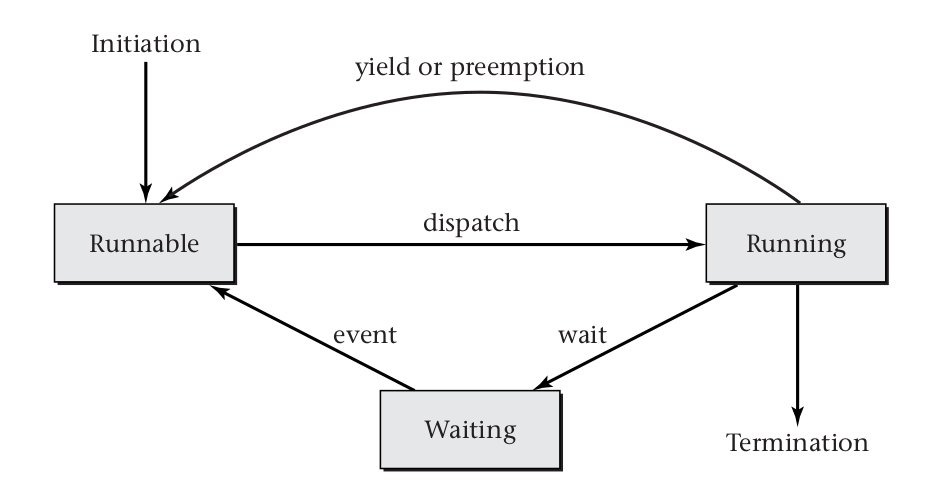
\includegraphics{img/scheduling_states.png}
  \end{itemize}
\end{itemize}

    \subsection{Scheduling goals}\label{scheduling-goals}

\begin{itemize}
\tightlist
\item
  \textbf{Throughput} is the rate which useful work is accomplished.

  \begin{itemize}
  \tightlist
  \item
    Example measure of throughput could be the number of search
    transactions per second
  \item
    Only by using all the I/O devices efficiently can a scheduler
    maximize throughput.
  \item
    Switching between threads more often than necessary will reduce
    throughput
  \item
    The thread runs best on the same processor, called \textbf{processor
    affinity}, because of cache therefore scheduling the same thread on
    the same core maximize throughput
  \item
    If a processor needs data from another processors cache it uses the
    systems \textbf{cache coherence protocol}

    \begin{itemize}
    \tightlist
    \item
      Typically means first transferring the data from the old cache to
      the main memory and then transferring it from the main memory to
      the new cache
    \end{itemize}
  \end{itemize}
\item
  \textbf{Response Time} is the elapsed time from a triggering event to
  to a completed response

  \begin{itemize}
  \tightlist
  \item
    A high performance system in throughput might be low performance in
    response time and vice versa
  \item
    System intended for direct interaction with a user tend to be
    optimized for response time whereas servers are optimized for
    throughput
  \item
    Often involves trade-offs between responding to different
    interactions

    \begin{itemize}
    \tightlist
    \item
      can be done by responding to the interaction which takes the
      smallest amount of time to complete

      \begin{itemize}
      \tightlist
      \item
        Called \textbf{Shortest Job First} (SJF)
      \item
        Normally a operating system does not know how much processor
        time each thread need to respond it often guess based on
        previous threads or based on previous burst
      \item
        \textbf{Burst} is the amount of processing done between waits
        for external events.
      \end{itemize}
    \item
      can also be done by frequently switching between threads
    \end{itemize}
  \end{itemize}
\item
  A task is \textbf{urgent} if it needs to be done soon
\item
  \textbf{Importance} indicate how much is at stake in accomplishing a
  task in a timely fashion.
\item
  \textbf{Resource Allocation} is how the resources are allocated
  between task

  \begin{itemize}
  \tightlist
  \item
    Is a matter of fairness
  \item
    \textbf{Proportional-share scheduling} balances the processing time
    given to threads over a much shorter time scale, such as a second.

    \begin{itemize}
    \tightlist
    \item
      The idea is to focus on the runnable threads and how much time the
      user has allocated to them
    \end{itemize}
  \item
    The niceness of a thread is akin to low priority.

    \begin{itemize}
    \tightlist
    \item
      Niceness on linux is interpret of the amount of processor time
    \item
      Niceness on OSX is interpret as thread with high niceness only get
      processor time when the processor is idle
      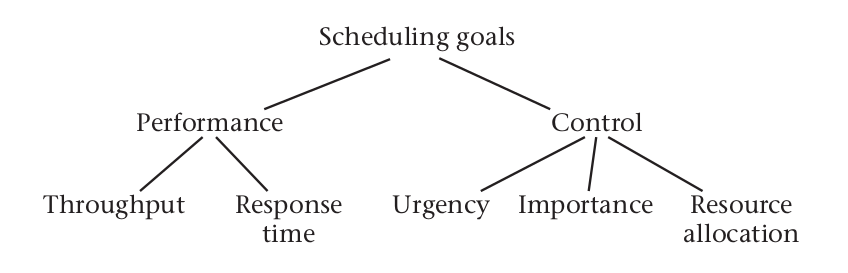
\includegraphics{img/scheduling_goals.png}
    \end{itemize}
  \end{itemize}
\end{itemize}

    \subsection{Scheduling Mechanisms}\label{scheduling-mechanisms}

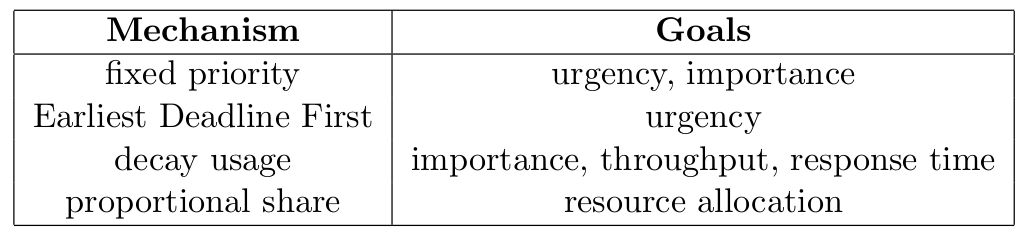
\includegraphics{img/scheduling_mechanisms_goals.png}
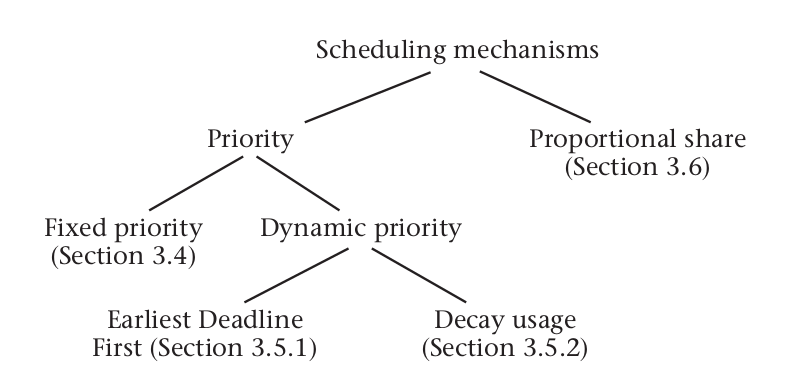
\includegraphics{img/scheduling_mechanisms.png}

    \subsubsection{Fixed-Priority
Scheduling}\label{fixed-priority-scheduling}

\begin{itemize}
\tightlist
\item
  Threads with higher priority runs before the onces with lower priority
\item
  A thread cannot change priority
\item
  In a fixed-priority scheduler the run queue can be kept in a
  data-structure ordered by priority

  \begin{itemize}
  \tightlist
  \item
    Typically represented as an array where the first entry contains a
    list of threads with highest priority the second entry contains a
    list of threads with the next highest priority, and so forth.
  \item
    Whenever a processor becomes idle because a thread has terminated or
    entered a waiting state, the scheduler dispatches a runnable thread
    of highest available priority.
  \item
    The processor also compares priorities if a thread becomes runnable

    \begin{itemize}
    \tightlist
    \item
      If the new thread has higher priority than the running thread the
      scheduler performs a thread switch
    \end{itemize}
  \item
    To deal with ties there are two possible solutions

    \begin{itemize}
    \tightlist
    \item
      Run the thread that become runnable first until it waits for some
      event of voluntarily yield the processor (first in, first out
      (FIFO))
    \item
      Share the processor between the threads that are tied in a
      \textbf{round-robin} fashion. (RR) \_\_\_\_
    \end{itemize}
  \end{itemize}
\item
  Not viable in a general purpose system
\item
  More suited for am environment where all the threads are part of a
  carefully quality-controlled system design.
\item
  Two key theorems make it easy to analyze a periodic hard-real-time
  system under fixed-priority scheduling:

  \begin{itemize}
  \tightlist
  \item
    If the threads meet their deadlines under any fixed priority
    assignment, then they will do so under an assignment that
    prioritizes threads with shorter periods over those with longer
    periods. This policy is known as \textbf{rate-monotonic scheduling.}
  \item
    To check that the deadlines are met it suffices to check the worst
    cast scenario where the threads start at the same time \_\_\_
  \end{itemize}
\item
  To test the feasibility of a real-time schedule, it is conventional to
  use a \textbf{Gantt chart}.

  \begin{itemize}
  \tightlist
  \item
    is a bar, which represent the passage of time, divided into regions
    labeled to show what thread is running during the corresponding time
    interval.
  \item
    can be used to check whether a rate-monotonic fixed priority
    schedule will work for a given set of threads
  \end{itemize}
\end{itemize}

    \subsubsection{Dynamic Priority
Scheduling}\label{dynamic-priority-scheduling}

\begin{itemize}
\tightlist
\item
  In \textbf{Earliest Deadline First Scheduling} each time a thread
  becomes runnable the priorities according to the following rule: the
  sooner a threads dealing the higher its priority
\item
  \textbf{Decay Scheduling} priority downward from the base priority by
  an amount that reflects recent processor usage by that thread.

  \begin{itemize}
  \tightlist
  \item
    The user-specified priorities can serve as base priorities, which
    the operating system will use as a starting point for its automatic
    adjustments.

    \begin{itemize}
    \tightlist
    \item
      Most of the time the users will use the default thread priorities
      for all their threads and threads only differ in priority because
      of the
    \item
      The threads that are a tie after automatic adjustment are
      processed in a round robin fashion
    \end{itemize}
  \item
    The time that each thread are allowed to run before switching is
    called a \textbf{quantum}

    \begin{itemize}
    \tightlist
    \item
      The priority will not sink below some minimum value
    \item
      If the thread has been running for a while it has a low priority
    \item
      If the thread has not run for a long time its priority will be
      equal to the base priority
    \end{itemize}
  \item
    The thread's recent processor usage increases when the thread runs
    and \textbf{decays} when the thread waits

    \begin{itemize}
    \tightlist
    \item
      The currently running thread has its usage updated whenever it
      voluntarily yields the processor\\
      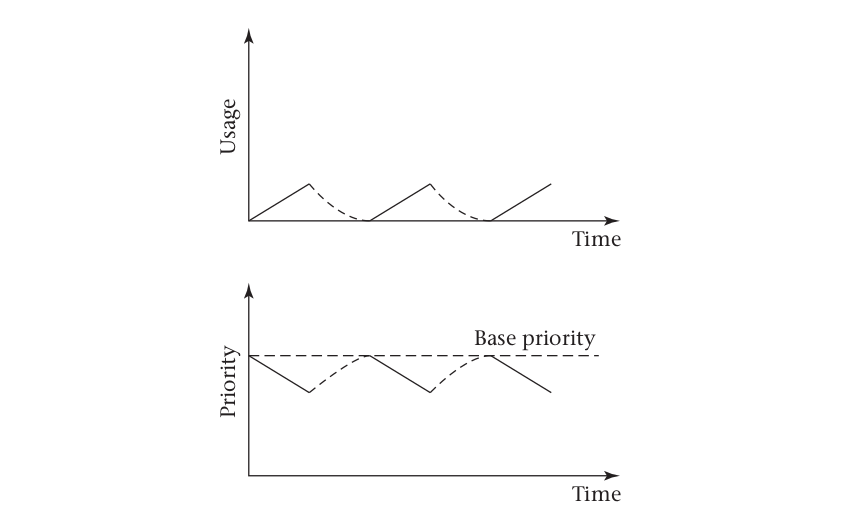
\includegraphics{img/decay_osx.png}
    \end{itemize}
  \end{itemize}
\end{itemize}

    \subsubsection{Proportional-Share
Scheduling}\label{proportional-share-scheduling}

\begin{itemize}
\tightlist
\item
  When resource allocation is the primary user-goal
\item
  Researchers have proposed three basic mechanisms for controlling the
  rate at which threads are granted processor time:

  \begin{enumerate}
  \def\labelenumi{\arabic{enumi}.}
  \tightlist
  \item
    Each thread can be granted the use of the processor equally often

    \begin{itemize}
    \tightlist
    \item
      Just as in simple round robin
    \item
      Those who have larger allocation and granted larger time slice
    \item
      Known as \textbf{Weighted Round Robin Scheduling} (WRR)
    \end{itemize}
  \item
    A uniform time slice can be used for all threads.

    \begin{itemize}
    \tightlist
    \item
      Those with larger allocations are run more often
    \item
      The smaller allocation sit out on some rotations through the list
    \item
      Several names are used

      \begin{itemize}
      \tightlist
      \item
        Weighted Fair Queuing (WFQ),
      \item
        Stride Scheduling
      \item
        Virtual Time Round-Robin Scheduling (VTRR).
      \end{itemize}
    \end{itemize}
  \item
    A uniform time slice can be used for all threads.

    \begin{itemize}
    \tightlist
    \item
      Those with larger allocations are chosen to be run more often
    \item
      The threads are selected by a lottery with weighted odds
    \item
      This is not terribly practical
    \item
      Known as \textbf{lottery scheduling}
    \end{itemize}
  \end{enumerate}
\end{itemize}

\begin{center}\rule{0.5\linewidth}{\linethickness}\end{center}

\begin{itemize}
\tightlist
\item
  The Linux system uses \textbf{Completely Fair Scheduler} which always
  run the thread which is behind on virtual runtime

  \begin{itemize}
  \tightlist
  \item
    Virtual runtime is calculated based on the niceness of a thread and
    multiplied with the scale
  \item
    If a thread has been non-runnable for a certain amount of time its
    virtual runtime is set forward so as to be only slightly less than
    the minimum virtual runtime of any of the previously runnable
    threads.
  \item
    The run queue is kept sorted in order of the runnable threads'
    virtual runtimes.

    \begin{itemize}
    \tightlist
    \item
      Represented as a red-black search three
    \end{itemize}
  \item
    The thread scheduler switches threads if one of the two following
    things happend

    \begin{itemize}
    \tightlist
    \item
      A threads time slice has expired
    \item
      A new thread enters the run queue
    \end{itemize}
  \end{itemize}
\end{itemize}

    \subsection{Security}\label{security}

\begin{itemize}
\tightlist
\item
  The kind of attack most relevant to scheduling is the denial of
  service (DoS) attack

  \begin{itemize}
  \tightlist
  \item
    Is an attack with the goal of preventing legitimate users of a
    system to be able to use it
  \item
    e.g. Given an urgent thread a low priority
  \item
    Because of systems with e.g. decay scheduling, an attacker must run
    many concurrent threads in order to drain off a significant fraction
    of the processor's time.
  \item
    A limit number of threads per users will constrain denial of service
    attacks without causing most users much hardship.
  \end{itemize}
\end{itemize}

    \section{Processes and Protection}\label{processes-and-protection}

\begin{itemize}
\tightlist
\item
  Most mainstream systems definition of a \textbf{process} are based on
  definitions that include the following:

  \begin{itemize}
  \tightlist
  \item
    \textbf{One or more threads}

    \begin{itemize}
    \tightlist
    \item
      Is often closely associated with one thread
    \item
      Some programs are designed to divide work between multiple threads
    \end{itemize}
  \item
    \textbf{Virtual memory accessible to those threads}

    \begin{itemize}
    \tightlist
    \item
      The mainstream protection approach is for each process to have its
      own virtual memory address shared by threads within that process
    \item
      The access rights are assigned to the process, not to the
      individual threads.
    \end{itemize}
  \item
    \textbf{Other access rights}

    \begin{itemize}
    \tightlist
    \item
      The process can either hold a specific \textbf{capability} (e.g.
      writing to a file) or a \textbf{credential} such as the
      identification of the user for whom the process is running
    \end{itemize}
  \item
    \textbf{Resource allocation context}

    \begin{itemize}
    \tightlist
    \item
      Limited resources are associated with a process for two reasons

      \begin{itemize}
      \tightlist
      \item
        The process's termination may serve to implicitly release some
        of the resources it is holding
      \item
        The process may be associated with a limited resource quota
      \end{itemize}
    \end{itemize}
  \item
    \textbf{Miscellaneous context}

    \begin{itemize}
    \item
      The operating system tracks a single current working directory per
      process
    \item
    \end{itemize}
  \end{itemize}
\end{itemize}

    \subsection{POSIX Process Management
API}\label{posix-process-management-api}

\begin{itemize}
\tightlist
\item
  All operating systems provide mechanisms for creating new processes,
  terminating existing processes, and performing related actions.
\item
  In the POSIX approach each process is identified by a \textbf{process
  ID number} which is a positive integer
\item
  Each process comes into existence through the forking of a parent
  process.

  \begin{itemize}
  \tightlist
  \item
    Except the first process that is started when the operating system
    starts running
  \item
    A process forks off a new process whenever one of the threads
    running in the parent procedure calls the \texttt{fork} procedure
  \item
    In the parent process the call to \texttt{fork} returns returns the
    process ID number of the child process

    \begin{itemize}
    \tightlist
    \item
      May be important to the parent if it want to exert some control
      over the child later or find out if the child terminates
    \end{itemize}
  \item
    The child process is in many regards a copy of the parent process

    \begin{itemize}
    \tightlist
    \item
      For protection purpose it has the same credentials as the parent
    \item
      The child has the the same capabilities for such purposes as
      access to files that have been opened for reading or writing
    \item
      The child contains a copy of the parents address space

      \begin{itemize}
      \tightlist
      \item
        The operating system does not need to copy each page of address
        space it just copies on write (COW)
      \end{itemize}
    \end{itemize}
  \item
    The child starts by calling the \texttt{fork} procedure

    \begin{itemize}
    \tightlist
    \item
      Fork returns a value of 0 in the child.
    \item
      The normal programming pattern is for any fork operation to be
      immediately followed by an if statement that checks the return
      value from fork.

      \begin{itemize}
      \tightlist
      \item
        That way the programming code can change behavior if it is a
        child
      \end{itemize}
    \item
      Failure is signaled by a negative value
    \item
      Used in Linux to start new programs
    \end{itemize}
  \end{itemize}
\item
  In order to wait for a child process the parent can use the
  \texttt{waitpid} procedure which takes three arguments

  \begin{itemize}
  \tightlist
  \item
    The first argument is the process id of the child for which the
    parent should wait
  \item
    The two other arguments can be 0 if the parent should just wait for
    the just process to finish
  \item
    If the child process has exited before the parent the
    \texttt{waitpid} command does not wait
  \item
    The operating system retains information about the terminated
    process until the parent waits for it.
  \item
    A terminated process that has not yet been waited for is known as a
    zombie.

    \begin{itemize}
    \tightlist
    \item
      Waiting for a zombie is known as reaping the zombie.
    \end{itemize}
  \end{itemize}
\item
  A program file can have a special set user ID (\texttt{setuid}) set on
  it

  \begin{itemize}
  \tightlist
  \item
    The process that executes it acquires the credential of the file's
    owner.
  \item
    The setuid mechanism provides an extremely general mechanism for
    granting access rights.
  \end{itemize}
\end{itemize}

    \subsubsection{Exec family}\label{exec-family}

\begin{itemize}
\tightlist
\item
  The POSIX standard includes six different procedures, any one of which
  can be used to load in a new program and start it running.

  \begin{itemize}
  \tightlist
  \item
    They are commonly called the \textbf{exec family} because they have
    names starting with exec,
  \item
    Each member must be given enough information to find the new program
    stored in a file and to provide the program with any arguments and
    environment variables it needs.
  \item
    The family members differ in exactly how the calling program
    provides this information.
  \item
    Because the family members are so closely related, most systems
    define only the \texttt{execve} procedure in the kernel of the
    operating system itself
  \item
    Only return if an error occurs, because if all is well the new
    program starts running without the possibility of reaching the old
    program
  \end{itemize}
\item
  \texttt{execl} is one of the simpler members of the exec family

  \begin{itemize}
  \tightlist
  \item
    The first argument specifies where the program is located e.g.
    \texttt{/bin/ps}
  \item
    The remaining string are the command line arguments e.g. \texttt{ps}
    and \texttt{axl}
  \item
    An inconvenience about \texttt{execl} is that the location of the
    program file is needed
  \end{itemize}
\item
  \texttt{execlp} does not need to know the location of the program file

  \begin{itemize}
  \tightlist
  \item
    can be given a filename and will search through the directories to
    find the program
  \item
    if used in combination with work in a program a new command can be
    executed
  \end{itemize}
\end{itemize}

    \section{Synchronization}\label{synchronization}

\begin{itemize}
\tightlist
\item
  In a \textbf{race} two threads use the same data structure without any
  mechanisms to ensure only one threads use the data structure at a
  time.

  \begin{itemize}
  \tightlist
  \item
    Can be avoided using \textbf{locks}
  \end{itemize}
\item
  \textbf{Mutual exclusion} is when a thread temporarily excludes other
  threads when running on data structures
\end{itemize}

    \subsection{Mutexes and Monitors}\label{mutexes-and-monitors}

\begin{itemize}
\tightlist
\item
  A programmer can arrange for exclusive access to a data structure by
  using a lock object associated with it

  \begin{itemize}
  \tightlist
  \item
    Only one thread can lock it at a time
  \item
    When a thread uses a lock, it \textbf{holds} the locks
  \end{itemize}
\item
  To support race prevention, operating systems and middleware generally
  provide \textbf{mutual exclusion locks}

  \begin{itemize}
  \tightlist
  \item
    Often called \textbf{Mutex} for short
  \end{itemize}
\end{itemize}

    \subsubsection{The Mutex API}\label{the-mutex-api}

\begin{itemize}
\item
  A mutex can be in to states locked or unlocked

  \begin{itemize}
  \tightlist
  \item
    Needs to operations for locking and unlocking
  \item
    When a thread use the lock operations on a locked mutex, it waits
    for the lock to be unlocked
  \item
    If more than one thread are waiting for a mutex to be unlocked only
    one can unlock it and the others will wait
  \item
    There may also be operations for checking if a mutex is locked and
    removing it from memory
  \end{itemize}
\item
  In the POSIX API \texttt{my\_mutex} can be declared to be a mutex and
  initialize with the default attributes as follows:

\begin{Shaded}
\begin{Highlighting}[]
\NormalTok{pthread_mutex_t my_mutex;}
\NormalTok{pthread_mutex_init(&my_mutex, }\DecValTok{0}\NormalTok{);}
\end{Highlighting}
\end{Shaded}
\item
  A thread that wants lock a mutex, operate on the associated data
  structure and then unlock the mutex would do the following:

\begin{Shaded}
\begin{Highlighting}[]
\NormalTok{pthread_mutex_lock(&my_mutex);}
\CommentTok{// operate on the protected data structure}
\NormalTok{pthread_mutex_unlock(&my_mutex);}
\end{Highlighting}
\end{Shaded}
\item
  Destroying a mutex can be done in the following procedure call

\begin{Shaded}
\begin{Highlighting}[]
\NormalTok{pthread_mutex_destroy(&my_mutex);}
\end{Highlighting}
\end{Shaded}
\item
  POSIX has a couple variants on \texttt{pthread\_mutex\_lock} which can
  be useful under particular circumstances

  \begin{itemize}
  \tightlist
  \item
    \texttt{pthread\_mutex\_trylock} will never wait to acquire a mutex
    but throw an error code immediately if unable to acquire the lock
  \item
    \texttt{pthread\_mutex\_timedlock} allows the programmer to specify
    the maximum waiting time

    \begin{itemize}
    \tightlist
    \item
      If the mutex cannot be acquired within that time the procedure
      returns an error code
    \end{itemize}
  \end{itemize}
\item
  Types of mutexes in the POSIX standard

  \begin{itemize}
  \tightlist
  \item
    \texttt{PTHREAD\ MUTEX\ DEFAULT}

    \begin{itemize}
    \tightlist
    \item
      If a thread tries to lock a mutex that it already holds or unlocks
      one it does not, all bets are off as to what will happen.
    \item
      The programmer has the responsibility for this never happening
    \item
      Different POSIX system may behave differently
    \end{itemize}
  \item
    \texttt{PTHREAD\ MUTEX\ ERROR\ CHECK}

    \begin{itemize}
    \tightlist
    \item
      If a thread tries to lock a mutex that it alreadyholds, or unlock
      a mutex that it doesn't hold, the operation returns an error code.
    \end{itemize}
  \item
    \texttt{PTHREAD\ MUTEX\ NORMAL}

    \begin{itemize}
    \tightlist
    \item
      If a thread tries to lock a mutex that it already holds it goes
      into a deadlock situation waiting for itself to unlock the thread
    \item
      If it tries to unlock a lock it does not hold all bets are off and
      each POSIX-compliant system is free to respond however it likes.
    \end{itemize}
  \item
    \texttt{PTHREAD\ MUTEX\ RECURSIVE}

    \begin{itemize}
    \tightlist
    \item
      If a thread tries to unlock a mutex it does not hold it returns an
      error code
    \item
      When a thread tries to lock a mutex it already holds it simple
      increments a counter and it is allowed to proceed, then when it
      unlocks it decrements the counter
    \end{itemize}
  \end{itemize}
\end{itemize}

    \subsubsection{Monitors}\label{monitors}

\begin{itemize}
\tightlist
\item
  In object oriented programming the mutex can be used in a very rigidly
  structured way:

  \begin{itemize}
  \tightlist
  \item
    All state variables within an object should be kept private and only
    accessible by the code within that object
  \item
    Every object should contain a mutex as an additional field
  \item
    Every method should start by locking that object's mutex and end by
    unlocking it before returning
  \end{itemize}
\item
  When the mutex rules are applied it will be impossible for two thread
  to race an objects state

  \begin{itemize}
  \tightlist
  \item
    An programming language can follow the mutex rules are the
    programmer can apply them manually
  \item
    An object that automatically follows the mutex rules are called a
    \textbf{monitor}.

    \begin{itemize}
    \tightlist
    \item
      e.g. in pascal using the keyword \texttt{monitor} or in java using
      the keyword \texttt{synchronized,}at the beginning of every
      non-private method
    \end{itemize}
  \end{itemize}
\end{itemize}

    \subsubsection{Underlying Mechanisms for
Mutexes}\label{underlying-mechanisms-for-mutexes}

\begin{itemize}
\tightlist
\item
  All modern processor architectures has at least one instruction that
  can be used to both change the contents of a memory location and get
  information about the previous contents of the location

  \begin{itemize}
  \tightlist
  \item
    These instructions are executed atomically
  \item
    One of them is called the \texttt{exchange} operation, which
    atomically swaps the contents of a register with the contents of a
    memory location
  \end{itemize}
\item
  \textbf{The basic spinlock}

  \begin{itemize}
  \tightlist
  \item
    It can be represented as a memory location that contains 1 if the
    mutex is unlocked and 0 if the mutex is locked
  \item
    The unlock operation can be trivial: to unlock a mutex just store 1
    into it
  \item
    The lock operation uses the atomically exchange operation where it
    swaps a 0 with 0 until it gets a 1

    \begin{itemize}
    \item
      Psuedo code

\begin{verbatim}
to lock mutex:
let temp = 0
repeat
    atomically exchange temp and mutex
until temp = 1
\end{verbatim}
    \end{itemize}
  \item
    Due to cache coherence the basic spin lock is very inefficient when
    two threads are waiting at the same time

    \begin{itemize}
    \tightlist
    \item
      To avoid this reads can be used instead an then when the mutex
      becomes unlock they try to grab it and is refered to as the
      \textbf{Cache-conscious spinlock}
    \end{itemize}
  \item
    A mutex that uses busy waiting is called a \textbf{spinlock}
  \end{itemize}
\item
  \textbf{The queuing lock}

  \begin{itemize}
  \tightlist
  \item
    Notifies the operating system that it needs to wait
  \item
    Notifying that the thread needs to wait requires some overhead

    \begin{itemize}
    \tightlist
    \item
      Therefore the relative efficiency of spinlocks and queuing locks
      depends on the time the lock waits
    \end{itemize}
  \item
    Used for cases where a thread might hold a mutex a long time
  \item
    Has three components

    \begin{itemize}
    \tightlist
    \item
      A memory location used to record the mutexs state, 1 for unlocked
      or 0 for locked
    \item
      A list of threads waiting to acquire the mutex

      \begin{itemize}
      \tightlist
      \item
        This list allows the scheduler to place the threads in a waiting
        state
      \end{itemize}
    \item
      A cache-conscious spinlock, used to protect against races in
      operations on the mutex ifself
    \end{itemize}
  \item
    The locked mutex is passed from one thread to another without being
    unlocked
  \end{itemize}
\end{itemize}

    \subsection{Other Synchronization
Patterns}\label{other-synchronization-patterns}

    \subsubsection{Bounded Buffers}\label{bounded-buffers}

\begin{itemize}
\tightlist
\item
  Often two threads are linked together in a processing
  \textbf{pipeline}

  \begin{itemize}
  \tightlist
  \item
    Where one thread (\textbf{producer}) produces output used by other
    thread (\textbf{consumer})
  \item
    Can be done using a a intermediate storage area called a
    \textbf{buffer}, where the producer places results and the consumer
    retrieve the result
  \item
    If the consumer tries to retrieve a value from and empty buffer it
    needs to wait for the producer to catch up
  \item
    If using a limited sized buffer (\textbf{bounded buffer}) the
    producer needs to wait if it gets to far ahead
  \item
    Found in the piping feature in UNIX:
    \texttt{ls\ \textbar{}\ tr\ a-z\ A-Z}
  \end{itemize}
\end{itemize}

    \subsubsection{Reader/Writers Locks}\label{readerwriters-locks}

\begin{itemize}
\tightlist
\item
  A \textbf{readers/writers lock} is much like a mutex excepts that when
  a thread lcosk the lock, it specifies whether it is planning to do any
  writing to the protected data structure or only reading

  \begin{itemize}
  \tightlist
  \item
    The lock operating like a mutex waits until the lock can be acquired
  \item
    Any number of readers can hold the lock at the same time
  \item
    Has a higher overhead than a mutex since a mutex is simpler
  \item
    To avoid starvation of waiting writers some versions of
    reader/writers locks make new readers wait until after the waiting
    writers
  \end{itemize}
\item
  The POSIX standard includes readers/writers locks

  \begin{itemize}
  \tightlist
  \item
    Used with procedures such as \texttt{pthread\_rwlock\_init},
    \texttt{pthread\_rwlock\_rdlock}, \texttt{pthread\_rwlock\_wrlock},
    and \texttt{pthread\_rwlock\_unlock}
  \item
    The POSIX standard leaves it up to each individual system how to
    priorities new readers versus waiting writers
  \item
    The POSIX standard also includes a more specialized form of
    readers/writers locks specifically associated with files

    \begin{itemize}
    \tightlist
    \item
      In the POSIX standard, file locks are available through the
      complex \texttt{fcnt} procedure
    \item
      Most UNIX-family OSs also provide a simpler interface,
      \texttt{flock}
    \end{itemize}
  \end{itemize}
\end{itemize}

    \subsubsection{Barriers}\label{barriers}

\begin{itemize}
\tightlist
\item
  \textbf{Barriers} are most commonly used in programs that do
  large-scale numerical calculations for scientific or engineering
  applications

  \begin{itemize}
  \tightlist
  \item
    May also be used in other application as long as there is a
    requirement for all threads in a group to finish one phase of the
    computation before any of the moves on to the next phase
  \end{itemize}
\item
  When a barrier is created, the programming specifies how many threads
  will be sharing it

  \begin{itemize}
  \tightlist
  \item
    Each of the threads completes the first phase of the computations
    and then invokes the barrier's wait operation
  \item
    When the last thread invokes the wait operation the wait operation
    immediately returns
  \item
    When the all the threads are done with the first phase they proceed
    to the second phase and the barrier is used again and for the
    remaining phases
  \item
    Barriers are provided as part of POSIX and other widely available
    APIs
  \end{itemize}
\end{itemize}

    \subsection{Condition Variables}\label{condition-variables}

\begin{itemize}
\tightlist
\item
  \textbf{Condition variables} can be used to help a thread wait until
  circumstances are appropriate for it to proceed

  \begin{itemize}
  \tightlist
  \item
    It works in partnership with monitors or with mutexes used in the
    style of monitors
  \item
    There are two basic operations on a condition variable \texttt{wait}
    and \texttt{notify}
  \item
    A thread that finds circumstances that are not to its liking invokes
    the wait command and goes to sleep until another thread invokes the
    notify command
  \item
    In Java each object has a single condition variable automatically
    associated with it

    \begin{itemize}
    \tightlist
    \item
      An objects \texttt{wait} method wait on the objects condition
      variable
    \item
      The \texttt{notifyAll} method wakes up all the threads waiting
    \end{itemize}
  \item
    When calling the \texttt{wait} the thread releases the lock so
    anther threads can use it
  \item
    The waiting needs to be done inside a while loop to ensure that the
    invariant is true
  \end{itemize}
\item
  The POSIX API allows multiple condition variable per mutex

  \begin{itemize}
  \tightlist
  \item
    They are initialized with \texttt{pthread\_cond\_init} independent
    of any particular mutex
  \item
    The mutex is passed as an argument to \texttt{pthread\_cond\_wait}
    with the condition variable being waited on
  \item
    The operations corresponding to \texttt{notify} and
    \texttt{notifyAll} are called \texttt{pthread\_cond\_signal} and
    \texttt{pthread\_cond\_broadcast} without holding corresponding
    mutex
  \end{itemize}
\end{itemize}

    \subsection{Semaphores}\label{semaphores}

\begin{itemize}
\tightlist
\item
  \textbf{Semaphores} are another synchronization mechanism with the
  same generality as monitors with condition variables

  \begin{itemize}
  \tightlist
  \item
    They are less natural, resulting in more error-prone code
  \item
    The applications where they are more natural e.g. bounded buffers
    they result in very succinct clear code
  \item
    Used before monitors
  \item
    Available in Java as the class \texttt{Semaphore} from the package
    \texttt{java.util.concurrent}
  \end{itemize}
\item
  A semaphore is essentialy an unsigned integer variable where only
  three operations are allowed:

  \begin{itemize}
  \tightlist
  \item
    At the time the semaphore is created, it may be initialized to any
    nonnegative integer of the programmers choice
  \item
    It may be increased by 1

    \begin{itemize}
    \tightlist
    \item
      The operation is called either \texttt{release}, \texttt{up} or
      \texttt{V}
    \end{itemize}
  \item
    It may be decreased by 1

    \begin{itemize}
    \tightlist
    \item
      The operation is called either \texttt{acquire}, \texttt{down} or
      \texttt{P}
    \item
      The thread performing an \texttt{acquire} operation waits if the
      value is 0.
    \item
      Only once another thread has performed a \texttt{release}
      operation to make the value positive does the waiting thread
      continue with its acquire operation
    \end{itemize}
  \end{itemize}
\item
  Semaphore can be used as mutexes

  \begin{itemize}
  \tightlist
  \item
    It should be initialized to one
  \item
    \texttt{acquire} is used as the ocking operation and
    \texttt{release} as unlocking
  \item
    can result it some nasty behavior if unlocked 2 times
  \end{itemize}
\item
  Semaphores can be used for keeping track of the available quantity of
  some resource, such as free spaces or data values in a bounded buffer

  \begin{itemize}
  \tightlist
  \item
    Whenever a thread creates a unit of the resource it increases the
    semaphores
  \item
    Whenever a thread wants to consume a unit of resource it first does
    an \texttt{acquire} on the semaphore
  \item
    It can be used e.g. on a \texttt{BoundedBuffer}
  \end{itemize}
\end{itemize}

    \subsection{Deadlocks}\label{deadlocks}

\begin{itemize}
\tightlist
\item
  A \textbf{deadlock} exists whenever there is a cycle of threads, each
  waiting for some resource held by the next under the following
  defining conditions

  \begin{enumerate}
  \def\labelenumi{\arabic{enumi}.}
  \tightlist
  \item
    Threads hold resources exclusively ("mutual exclusions")
  \item
    Threads hold some resources while waiting for additional ones ("wait
    for")
  \item
    Resources cannot be removed from threads forcibly ("No preemption")
  \item
    Threads wait in a circular chain such that each thread holds
    resources that are requested by the next thread in the chain
  \end{enumerate}
\item
  Deadlocks are quite rare even if measures are taken to avoid them
\end{itemize}

    \subsubsection{Resource Ordering (Deadlock
prevention)}\label{resource-ordering-deadlock-prevention}

\begin{itemize}
\tightlist
\item
  The ideal way to cope with deadlocks is preventing them from happening

  \begin{itemize}
  \tightlist
  \item
    \textbf{Deadlock prevention} aims to ensure that at least one of the
    four defining conditions is not satisfied
  \end{itemize}
\item
  One way of deadlock prevention targets the circular wait situation
  which is characterized by condition 4 by imposing a linear order in
  which resources need to be locked

  \begin{itemize}
  \tightlist
  \item
    Ordered by memory location
  \item
    Can only be done if the locks needed are known
  \end{itemize}
\end{itemize}

    \subsubsection{Ex Post Facto (Deadlock
detection)}\label{ex-post-facto-deadlock-detection}

\begin{itemize}
\tightlist
\item
  To detect a deadlock information about who is waiting for whom is
  needed

  \begin{itemize}
  \tightlist
  \item
    Can be done by keeping mutex records not just whether it is locked
    or unlocked but also which thread it is held by if any and which
    threads are waiting for it
  \end{itemize}
\item
  With information about who is waiting for whom a \textbf{resource
  allocation graph} can be constructed

  \begin{itemize}
  \tightlist
  \item
    Threads are represented as squares.
  \item
    Mutexs are represented as circles
  \item
    The arrows shod which mutex each thread is waiting to acquire and
    which thread each mutex is currently held by
  \item
    If a graph has a cycle it means that the system is deadlocked
  \end{itemize}
\item
  A system can test for deadlocks periodically or when a thread has
  waited an unreasonable long time for a lock

  \begin{itemize}
  \tightlist
  \item
    To test for a deadlock the system uses a standard graph algorithm to
    check whether the resource allocation graph contains a cycle
  \item
    Since a mutex out-degree can be greater than one a simple graph
    search can be used
  \end{itemize}
\item
  When a deadlock is detected, one of the deadlocked threads must be
  forcible terminated or rolled back to an earlier state to free up
  mutexes

  \begin{itemize}
  \tightlist
  \item
    Ex Post Facto is not commonly used in general purpose operating
    system because of this, but can be useful in a database system
  \end{itemize}
\end{itemize}

    \subsubsection{Immediate Deadlock
Detection}\label{immediate-deadlock-detection}

\begin{itemize}
\tightlist
\item
  \textbf{Immediate deadlock detection} is intervening at the very
  moment when the system would otherwise deadlock

  \begin{itemize}
  \tightlist
  \item
    As long as the deadlock is not allowed to occur the resource
    allocation graph will remain acyclic
  \end{itemize}
\item
  Each time a thread tries to lock a mutex, the system can act as
  follows

  \begin{itemize}
  \tightlist
  \item
    If the mutex is unlocked, lock it and add an edge from the mutex to
    the thread, to indicate that the thread holds the lock
  \item
    If the mutex is locked follow the chain of edges from it until the
    chain ends is the end of the chain the same as the thread trying to
    lock the mutex

    \begin{itemize}
    \tightlist
    \item
      If not add an edge showing that the thread is waiting for the
      mutex and put the thread into a waiting state
    \item
      If the end of the chain is the same thread, adding the extra edge
      would complete the cycle

      \begin{itemize}
      \tightlist
      \item
        Do not add the edge and do not put the thread into a waiting
        state
      \item
        Return an error code from the lock request or throw an exception
        indicate that the mutex could not be locked because an deadlock
        would have results
      \end{itemize}
    \end{itemize}
  \end{itemize}
\item
  When a possible deadlock is detected the program release all locks it
  currently holds and restart

  \begin{itemize}
  \tightlist
  \item
    The chance of repeating the response can be reduced by sleeping
  \end{itemize}
\item
  Used in \texttt{fcntl} in Linux and Mac OS for file locks
\end{itemize}

    \subsection{The Interaction of Synchronization with
Scheduling}\label{the-interaction-of-synchronization-with-scheduling}

\begin{itemize}
\tightlist
\item
  Synchronization and scheduling interact with one another

  \begin{itemize}
  \tightlist
  \item
    Since the scheduler controls which runnable thread runs on each
    processor and synchronization actions preformed by the running
    thread controls which threads are runnable
  \end{itemize}
\end{itemize}

    \subsubsection{Priority Inversion}\label{priority-inversion}

\begin{itemize}
\tightlist
\item
  If threads of different priority levels share mutexes or other block
  synchronization primitives, some minor violations of priority ordering
  are inevitable

  \begin{itemize}
  \tightlist
  \item
    A low priority having a mutex while a high priority one waits for it
    is generally no a big violation because programmers ensure that
    threads does not holds mutexes for very long
  \end{itemize}
\item
  \textbf{Priority Inversion} occurs when a low priority holds a mutex
  that a high priority thread needs and then when then medium priority
  thread runs in stead keeping the high-priority from running because
  the low priority one cannot run

  \begin{itemize}
  \tightlist
  \item
    A solution is to avoid fixed priority scheduling and use a decay one
    instead
  \item
    The genuine solution is \textbf{priority inheritance}.

    \begin{itemize}
    \tightlist
    \item
      Any thread that is waiting for a mutex temporarily lends its
      priority to the thread that holds the mutex
    \item
      A thread that holds mutexes runs with the highest priority among
      its own priority and those priorities it has been lend by the
      other threads waiting for the mutex
    \end{itemize}
  \end{itemize}
\end{itemize}

    \subsubsection{The Convoy Phenomenon}\label{the-convoy-phenomenon}

\begin{itemize}
\tightlist
\item
  The queue of threads in a popular mutex is names the \textbf{convoy}

  \begin{itemize}
  \tightlist
  \item
    This causes threads which holds the mutex to runs for a time slice
    and then stop when trying to acquire the mutex again
  \item
    Creates a long queue where each thread in turn moving from the front
    of the mutex through a brief period of execution and back to the
    rear of the queue
  \item
    This causes to problems two problems

    \begin{itemize}
    \tightlist
    \item
      The context switching rate goes up. I

      \begin{itemize}
      \tightlist
      \item
        Instead of one context switch pr time slice there is one per
        attempt to acquire the popular mutex
      \item
        The overhead of all tge context switches will affect the
        throughput
      \end{itemize}
    \item
      The scheduler's policy for choosing which thread to run is
      subverted

      \begin{itemize}
      \tightlist
      \item
        This can be avoided by handling the mutex wait queue in priority
        order the same way as the run queue
      \end{itemize}
    \end{itemize}
  \item
    It can be avoided by making all the threads runnable and unlocking
    the mutex
  \item
    The POSIX stanard API for mutexes requires that one or the other of
    the two prioritization-preserving approaches to be takes
  \end{itemize}
\end{itemize}

    \subsection{Nonblocking
Synchronization}\label{nonblocking-synchronization}

\begin{itemize}
\tightlist
\item
  To an unblocking version of a set function can use the compare-and-set
  instruction meets this need by doing the following two things
  atomically (Java example: \texttt{AtomicReference} in
  \texttt{java.util.concurrent.atomic} package) .:

  \begin{enumerate}
  \def\labelenumi{\arabic{enumi}.}
  \tightlist
  \item
    The instruction determines whether a variable contains a specified
    value and reports the answer
  \item
    The instruction sets the variable to a new value, but only if the
    answer to the preceding question was yes
  \end{enumerate}
\item
  It can be done until successful
\end{itemize}

    \section{Network overview}\label{network-overview}

    \subsection{Layers}\label{layers}

\begin{itemize}
\tightlist
\item
  LANs, IP and TCP are often called \textbf{layers}

  \begin{itemize}
  \tightlist
  \item
    They constitute the Link layer, the Internet work layer and
    Transport layer respectively
  \item
    Together with the application layer they form the
    \textbf{"four-layer model"} for networks
  \end{itemize}
\item
  The LAN layer is in charge of actual delivering a packets, using LAN
  supplied addresses

  \begin{itemize}
  \tightlist
  \item
    Is often subdivided into the physical layer dealing with the e.g.
    radio signals and mechanisms involved and above it and abstracted
    logical LAN layer that describes the digital non-analog operations
    on packages
  \item
    If divided gives us a five-layer model
    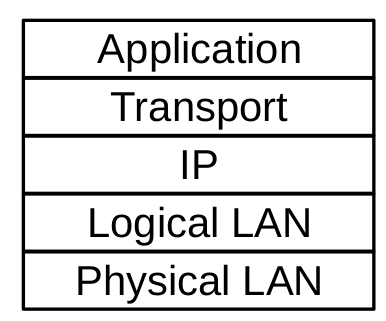
\includegraphics{img/network_layers.png}
  \end{itemize}
\end{itemize}

    \subsection{Data Rate, Throughput and
Bandwidth}\label{data-rate-throughput-and-bandwidth}

\begin{itemize}
\tightlist
\item
  Any network connection e.g. the LAN layer has a \textbf{data rate}

  \begin{itemize}
  \tightlist
  \item
    The rate which bits are transmitted
  \item
    The data rate can vary with time in some LANs e.g. Wi-Fi
  \end{itemize}
\item
  \textbf{Throughput} refers to the overall effective transmission rate

  \begin{itemize}
  \tightlist
  \item
    Taking into account into account things like transmission overhead,
    protocol ineffectiveness and perhaps even competing traffic
  \item
    Is generally measured a network layer than data rate
  \end{itemize}
\item
  \textbf{Bandwidth} can refer to either data rate or throughput

  \begin{itemize}
  \tightlist
  \item
    Mostly used for data rate (in the book)
  \end{itemize}
\item
  The term \textbf{goodput} is used to refer to the "application layer
  throughput" when talking about TCP

  \begin{itemize}
  \tightlist
  \item
    The amount of usable data being delivered to the receiving
    application
  \end{itemize}
\item
  Data rates are generally calculated in kilobits per second (Kbps) or
  megabits per second (Mbps); the use of lowercase "b" denotes bits

  \begin{itemize}
  \tightlist
  \item
    In the context of data rates, a kilobit is \(10^3\) bits (not
    \(2^{10}\) ) and a megabit is \(10^6\) bits
  \end{itemize}
\end{itemize}

    \subsection{Packets}\label{packets}

\begin{itemize}
\item
  Packets are a modest-sized buffer, transmitted as a unit through some
  shared set of links

  \begin{itemize}
  \tightlist
  \item
    Packets needs to be prefixed with a \textbf{header} containing
    delivery information
  \item
    The the common case known as \textbf{datagram forwarding}, the
    header contains a destination \textbf{address}
  \item
    Headers in networks using \textbf{virtual-circuit} forward contain
    an indentifier for the connection
  \item
    Almost all networking today are packet based
  \end{itemize}
\item
  At the LAN layer, packets can be viewed as the imposition of a buffer
  (and addressing) structure on top of low-level serial lines

  \begin{itemize}
  \tightlist
  \item
    Additional layers then impose additional structure
  \item
    Packets are often referred to as \textbf{frames} at the LAN layer
    and as \textbf{segments} at the Transport layer
  \end{itemize}
\item
  The max packet size supported by a given LAN is an intrinsic attribute
  of that LAN

  \begin{itemize}
  \tightlist
  \item
    Ethernet allows a maximum of 1500 bytes of data
  \end{itemize}
\item
  Each layer adds its own header
\item
  In datagram-forwarding networks the appropriate header will contain
  the address of the destination and perhaps other delivery information

  \begin{itemize}
  \tightlist
  \item
    Internal nodes of the network called \textbf{routers} or
    \textbf{switches} try to ensure that the packet are delivered to the
    requested destination
  \end{itemize}
\end{itemize}

    \subsection{Datagram Forwarding}\label{datagram-forwarding}

\begin{itemize}
\tightlist
\item
  In the datagram-forwarding model of packets delivery, packet headers
  contain a destination address.

  \begin{itemize}
  \tightlist
  \item
    It is up to the intervening switches or routers to look at this
    address and get the packets to the correct destination
  \item
    It used both by Ethernet switches and by IP routers l
  \end{itemize}
\item
  Delivering is achieved by providing each switch with a forwarding
  table of \(\langle\)destination,next\_hop\(\rangle\) pairs.

  \begin{itemize}
  \tightlist
  \item
    When a packet arrived the switch looks up the destination address in
    its forwarding table and finds the \textbf{next\_hop} information:

    \begin{itemize}
    \tightlist
    \item
      the immediate-neighbor address to which the packet should be
      forwarded to bring it closer to the destination
    \end{itemize}
  \item
    The next\_hop value in the forwarding table is a single entry; each
    switch is only responsible for a single step in the switch bath
  \item
    The destination entries in the forwarding table do not have to
    correspond exactly with the packet destination address

    \begin{itemize}
    \tightlist
    \item
      They do for ethernet datagram forwarding
    \item
      In IP routing, the table destination correspond to
      \textbf{prefixes} of IP addresses
    \end{itemize}
  \item
    The fundamental requirement is that a switch can determine the next
    hop using its forwarding table and destination address in the
    arriving packet
  \item
    Is also called \textbf{stateless} forwarding
  \item
    IP routers commonly as a \textbf{default} entry matching any
    nonlocal IP addresses
  \end{itemize}
\item
  The fundamental alternative is \textbf{virtual circuts}

  \begin{itemize}
  \tightlist
  \item
    Each router maintains state about each connection passing through
    it,
  \end{itemize}
\end{itemize}

    \section{Ethernet}\label{ethernet}

    \subsection{10-Mbps Classic Ethernet}\label{mbps-classic-ethernet}

\begin{itemize}
\tightlist
\item
  The Ethernet originally consisted of a long cable and when a station
  transmitted data went everywhere along the cable

  \begin{itemize}
  \tightlist
  \item
    Is known as a \textbf{broadcast bus}
  \item
    All packets were on the physical layer, broadcast onto a shared
    medium and could be seen by all other nodes
  \item
    The \textbf{network interface} took care of the details of
    transmitting, receiving and deciding which packet should be
    forwarded to the host via CPU interrupt

    \begin{itemize}
    \tightlist
    \item
      Made it appear logically as peer-to-peer
    \end{itemize}
  \end{itemize}
\item
  If to stations transmitted as the same time both signals would
  \textbf{collide} and fail as a result

  \begin{itemize}
  \tightlist
  \item
    In order to minimize collision loss, each station would implement
    the following

    \begin{enumerate}
    \def\labelenumi{\arabic{enumi}.}
    \tightlist
    \item
      Before the transmission wait for the line to become quite
    \item
      While transmitting continually monitor the line for signs that a
      collision has occurred; if a collision is detected cease
      transmitting
    \item
      If a collision occurs, use backoff-and-retransmit strategy
    \end{enumerate}
  \item
    The collision avoidance properties can be summarized with the
    \textbf{CSMA/CD} acronym: Carrier Sense, Multiple Access, Collision
    Detect.
  \end{itemize}
\item
  Errors can occur

  \begin{itemize}
  \tightlist
  \item
    when packets have bits flipped or garbled by electrical noise on the
    cable

    \begin{itemize}
    \tightlist
    \item
      Ethernet package contain a 32-bit CRC error-detecting code to
      detect bit errors
    \end{itemize}
  \item
    when the package is be misaddressed by the sending host or if they
    arrive
  \end{itemize}
\end{itemize}

    \subsubsection{Ethernet Packet Format}\label{ethernet-packet-format}

\begin{itemize}
\tightlist
\item
  The format of a typical Ethernet packet, which is still used for
  newer, faster Ethernets: 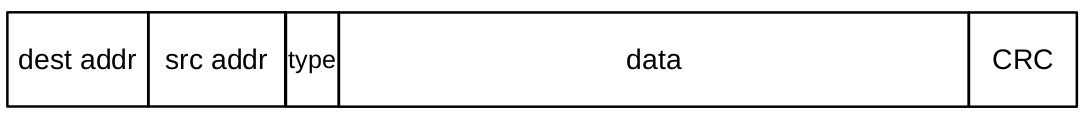
\includegraphics{img/ethernet_format.png}

  \begin{itemize}
  \tightlist
  \item
    The destination and source addresses are 48-bit quantities
  \item
    The type is 16-bits

    \begin{itemize}
    \tightlist
    \item
      Identifies the higher protocol layer
    \end{itemize}
  \item
    The data length is a variable up to a maximum of 1500 bytes\\
  \item
    The CRC checksum is 32-bits

    \begin{itemize}
    \tightlist
    \item
      Added by the Ethernet hardware, never by host software
    \end{itemize}
  \item
    There are also a preamble, which is a block of 1 bits followed by a
    0, in front of the packet for synchronization
  \item
    Each ethernet card has it own hardware address used for
    identification
  \end{itemize}
\end{itemize}

    \subsubsection{Ethernet Multicast}\label{ethernet-multicast}

\begin{itemize}
\tightlist
\item
  Another category of Ethernet addresses are \textbf{multicast}

  \begin{itemize}
  \tightlist
  \item
    Used to transmit a set of stations
  \item
    The lowest order bit of the first byte of the address indicates
    whether an address is physical or multicast
  \item
    To receive packets address to a given multicast address the host
    must inform the network interface that it wishes to do so

    \begin{itemize}
    \tightlist
    \item
      Once done any arriving packets addressed to that multicast address
      are forwarded to the host
    \end{itemize}
  \item
    The set of subscribers to a given multicast address is called a
    \textbf{multicast group}
  \item
    If several host subscribe to the same multicast address they each
    receive a copy of each multicast packet transmitted
  \item
    If switches are involved they normally forward multicast packages or
    broadcast packages on all outbound links
  \end{itemize}
\item
  All the cases in which a network interface forwards a received packet
  up to its attached host:

  \begin{itemize}
  \tightlist
  \item
    if the destination address of the received packet matches the
    physical address of an interface
  \item
    if the destination address of the received package is a broadcast
    address
  \item
    if the interface is in promiscuous mode (receive all packages)
  \item
    if the destination address of the received packet is a multicast
    address and the host has told the network interface to accept
    packets sent to that multicast address
  \end{itemize}
\end{itemize}

    \subsubsection{Ethernet Address Internal
Structure}\label{ethernet-address-internal-structure}

\begin{itemize}
\tightlist
\item
  The second-to-lowers-order bit of a physical Ethernet address
  indicates whether the address is believed to be globally unique or if
  its only locally unique

  \begin{itemize}
  \tightlist
  \item
    Known as the \textbf{Universal/Local} bit
  \item
    For real Ethernet physical address, the multicast and
    universal/local bits of the first byte should be 0
  \item
    Global Ethernet IDs are assigned to the physical Ethernet card by
    the manufacture

    \begin{itemize}
    \tightlist
    \item
      The first three bytes serve indicate the manufacture
    \end{itemize}
  \end{itemize}
\end{itemize}

    \subsubsection{The LAN Layer}\label{the-lan-layer}

\begin{itemize}
\tightlist
\item
  The LAN layer,

  \begin{itemize}
  \tightlist
  \item
    at its upper end, supplies to the network layer a mechanisms for
    addressing a package a sending it from one station to another
  \item
    at its lower end handles interactions with the physical layer
  \item
    covers packet addressing, delivery and receipt, forwarding, error
    detection, collision detection and collision-related retransmission
    attempts
  \item
    is divided into the \textbf{media access control}, or MAC, sublayer
    and a higher \textbf{logical link control} or LLC sublayer for
    higher-level flow-control functions that today have moved largely to
    the transport layer

    \begin{itemize}
    \tightlist
    \item
      The MAC layer is oftest used since it has the most frequently used
      functions
    \item
      LAN layer addresses are often called MAC addresses
    \end{itemize}
  \end{itemize}
\end{itemize}

    \subsubsection{The Slot Time and
Collisions}\label{the-slot-time-and-collisions}

\begin{itemize}
\tightlist
\item
  The \textbf{diameter} of an Ethernet is the maximum distance between
  any pair of stations

  \begin{itemize}
  \tightlist
  \item
    The maximum allowed diameter, measured in bits is limited to 232,
    which makes the round-trip-time 464 bits
  \item
    If a station involved in a collision discovers a it, it transmit a
    special \textbf{jam signal} of up to 48 bits
  \item
    The time to send 512 bits is the \textbf{slot time} of an Ethernet

    \begin{itemize}
    \tightlist
    \item
      Often described in bit times but in in conventional time units the
      slot time is 51.2 µsec.
    \end{itemize}
  \item
    If a station has transmitted for one slot time it is said to
    \textbf{acquired} the network

    \begin{itemize}
    \tightlist
    \item
      No collision can occur since any other station had has enough time
      to find out that the first station is transmitting
    \end{itemize}
  \item
    The Ethernet has a \textbf{minimum package size} equal to the slot
    time

    \begin{itemize}
    \tightlist
    \item
      A station transmitted that package are assured that is a collision
      were to occur, the sender would detect it and apply the
      retransmission algorithm
    \end{itemize}
  \item
    The Ethernet has a \textbf{maximum} packet size, of 1500 bytes

    \begin{itemize}
    \tightlist
    \item
      It is primarily for the sake of fairness
    \end{itemize}
  \end{itemize}
\end{itemize}

    \subsubsection{Exponential Backoff
Algorithm}\label{exponential-backoff-algorithm}

\begin{itemize}
\tightlist
\item
  Whenever there is a collision the Exponential Backoff Algorithm
  operating at the MAC layer is used to determine when each station will
  retry its transmission\\
\item
  The full Ethernet transmission algorithm

  \begin{enumerate}
  \def\labelenumi{\arabic{enumi}.}
  \tightlist
  \item
    Listen before transmitting ("carrier detect")
  \item
    If line is busy, wait for sender to stop and then wait an additional
    9.6 microseconds (96 bits).

    \begin{itemize}
    \tightlist
    \item
      One consequence of this is that there is always a 96-bit gap
      between packets, so packets do not run together.
    \end{itemize}
  \item
    Transmit while simultaneously monitoring for collisions
  \item
    If a collision does occur, send the jam signal and choose a backoff
    time as follows

    \begin{itemize}
    \tightlist
    \item
      For transmission \(N\), \(1\leq N \leq 10\) choose \(k\) randomly
      with \(0 \leq k < 2^N\). Wait \(k\) time slots times, check if
      line is idle, waiting if necessary for someone else to finish and
      then retry step 3. For \(10 \leq N \leq 15\) choose k randomly
      with \(0 \leq k < 2^10\)
    \end{itemize}
  \item
    If we reach \(N = 16\) give up
  \end{enumerate}
\item
  A problem that can occur when using the exponential Backoff Algorithm
  is the \textbf{Capture effect}

  \begin{itemize}
  \tightlist
  \item
    Is a potential lack of fairness
  \item
    Happens when one device is lucky a gets the line most when the other
    is trying to send the first package
  \end{itemize}
\end{itemize}

    \subsubsection{CSMA persistence}\label{csma-persistence}

\begin{itemize}
\tightlist
\item
  A carrier-sense/multiple-access transmission strategy is said to be
  \textbf{nonpersistent} if when the line is busy it waits a randomly
  selected time
\item
  A strategy is said to be \textbf{p-persistent} if, after waiting for
  the line to clear, the sender sends with probability \(p\leq 1\)
\item
  The ethernet uses 1-persistent

  \begin{itemize}
  \tightlist
  \item
    A consequence of this is that if more than one device are waiting
    for the line to clear a collision is certain
  \item
    Ethernet handles gracefully a resulting collision via the usual
    exponential backoff
  \end{itemize}
\end{itemize}

    \subsection{Ethernet Learning
Algorithm}\label{ethernet-learning-algorithm}

\begin{itemize}
\tightlist
\item
  The solution for a switch to act as a drop-in replacement for a hub is
  to start out with an empty forwarding table and the incremently build
  the table to a learning process

  \begin{itemize}
  \tightlist
  \item
    If a switch does not have an entry for a particular destination, it
    will \textbf{fall back to flooding}

    \begin{itemize}
    \tightlist
    \item
      It will forward the packet out every interface other than the one
      which it arrived
    \end{itemize}
  \item
    A switch learns address locations as follows

    \begin{itemize}
    \tightlist
    \item
      For each interface, the switch maintains a table of physical (MAC)
      addresses that have appeared as source addresses in packets
      arriving via that interface
    \item
      When a package arrives on interface \(I\) with source address
      \(S\) and destination unicast address \(D\), the switch enters
      \(\langle S, I \rangle\) into its forwarding table
    \end{itemize}
  \item
    To deliver a packet, the switch also looks up the destination \(D\)
    in the forwarding table.

    \begin{itemize}
    \tightlist
    \item
      If an entry \(\langle D,J \rangle\) with \(J \ne I\) exists the
      switch \textbf{forwards} the packet out interface \(J\)
    \item
      If an entry \(\langle D,J \rangle\) with \(J = I\) exists the
      packet does not get forwarded at all
    \item
      If there is no entry for \(D\) the switch must flood the package
      out all interface \(J\) with \(J\ne I\)
    \end{itemize}
  \item
    After a while the fallback-to-flooding alternative is needed less
    and less often
  \end{itemize}
\end{itemize}

    \subsection{Spanning Tree Algorithm and
Redudancy}\label{spanning-tree-algorithm-and-redudancy}

\begin{itemize}
\tightlist
\item
  Used to avoid loops
\item
  The switch with the lowest id is the root
\item
  To create the spanning three it disable all the interfaces not
  following the following rules:

  \begin{enumerate}
  \def\labelenumi{\arabic{enumi}.}
  \tightlist
  \item
    It enables the port via which it reaches the root
  \item
    It enables any of its ports that further-out switches use to reach
    the root
  \item
    If a remaining port connects to a segment to which other
    ``segment-neighbor'' switches connect as well, the port is enabled
    if the switch has the minimum cost to the root among those
    segment-neighbors, or, if a tie, the smallest ID among those
    neighbors, or, if two ports are tied, the port with the smaller ID.
  \item
    If a port has no directly connected switch-neighbors, it presumably
    connects to a host or segment, and the port is enabled. Rules 1 and
    2 construct the spanning tree; if S3 reaches the root via S2, then
    Rule 1 makes sure S3's port
  \end{enumerate}
\end{itemize}

    \section{Packets}\label{packets}

    \subsection{Packet Delay}\label{packet-delay}

\begin{itemize}
\tightlist
\item
  There are several contributing sources to the packet delay

  \begin{itemize}
  \tightlist
  \item
    On LAN the most significant is \textbf{bandwidth delay}

    \begin{itemize}
    \tightlist
    \item
      The time needed for a sender to get onto the wire
    \item
      This is simply the packet size divided by the bandwidth
    \end{itemize}
  \item
    There is also \textbf{propagation delay}

    \begin{itemize}
    \tightlist
    \item
      This relates to the propagation of the bits at the speed of light
    \item
      This delay is the distance divided by the speed of light
    \end{itemize}
  \item
    The introduction of switches leads to \textbf{store-and-forward
    delay},

    \begin{itemize}
    \tightlist
    \item
      The time reading the packet before any of it can be retransmitted
    \end{itemize}
  \item
    A switch may also introduce \textbf{queuing delay}
  \end{itemize}
\end{itemize}

    \subsection{Error Detection}\label{error-detection}

\begin{itemize}
\tightlist
\item
  The basis strategy for error detection is to add some extra bits
  formally known as \textbf{error-detection code}, that will allow the
  receiver to determine is the packet has been corrupted in transit

  \begin{itemize}
  \tightlist
  \item
    A corrupted package will be discarded by the receiver
  \item
    Packet errors generally fall into two categories:

    \begin{itemize}
    \tightlist
    \item
      low-frequency bit errors due to things like cosmic rays, and
      interference errors, typically generated by nearby electrical
      equipment.
    \item
      Errors of the latter type generally occur in bursts, with multiple
      bad bits per packet. Occasionally, a malfunctioning network device
      will introduce bursty errors as well.
    \end{itemize}
  \end{itemize}
\end{itemize}

    \section{IP Version 4}\label{ip-version-4}

\begin{itemize}
\tightlist
\item
  IP has a better scalability than LAN
\item
  The IP network service should act like a giant LAN
\item
  To support package size higher than what LAN allows the IP protocol
  supports \textbf{fragmentation}

  \begin{itemize}
  \tightlist
  \item
    Breaks a large package into units that it can transport successfully
  \end{itemize}
\end{itemize}

    \subsection{The IPv4 Header}\label{the-ipv4-header}

\begin{itemize}
\tightlist
\item
  The IPv4 header needs to contain the following information:

  \begin{itemize}
  \tightlist
  \item
    destination and source address
  \item
    indication of ipv4 vs ipv6
  \item
    a Time To Live (TTL) value to prevent infinite routing loops
  \item
    a field indicating that comes next in the packet (e.g. TCP v UDP)
  \item
    fields supporting fragmentation and reassembly.
  \end{itemize}
\item
  The header is organized as a series of 32-bit words as follows :
  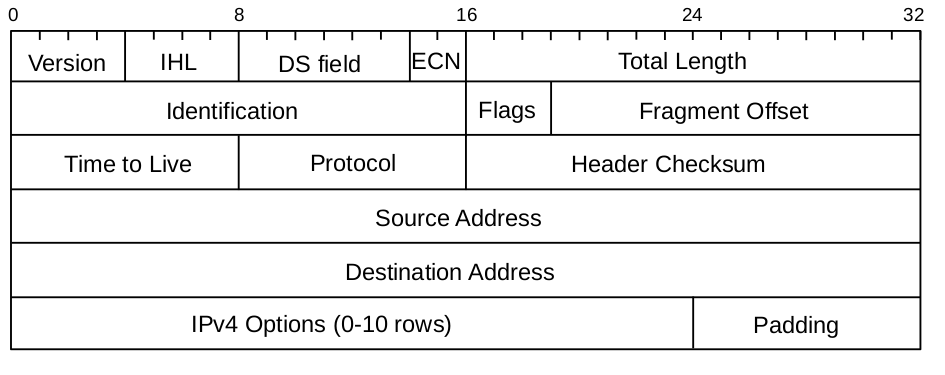
\includegraphics{img/ipv4_header.png}

  \begin{itemize}
  \tightlist
  \item
    The \textbf{Version} field is, for IPv4, the number 4: 0100
  \item
    The \textbf{IHL} field represents the total IPv4 Header Length in
    32-bit words

    \begin{itemize}
    \tightlist
    \item
      an IPv4 Header can thus be at most 15 words long
    \item
      The base header takes up five words, so the IPv¤ Options can
      consist of at most ten words.
    \end{itemize}
  \item
    The \textbf{Dofferential Services} (DS) field is used by the
    Differentiated Services suite to specify preferential handling for
    designated packets

    \begin{itemize}
    \tightlist
    \item
      e.g. those involved in VoIP or other real-time protocols
    \end{itemize}
  \item
    The \textbf{Explicit Congestion Notification} bits are there to
    allow router experiencing congestion to mark packets

    \begin{itemize}
    \tightlist
    \item
      This indicates to the sender that the transmission rate should be
      reduced
    \end{itemize}
  \item
    The \textbf{Total Length} field is present because an IPv¤ packet
    may be smaller than the minimum LAN packet size or larger than thewe
    maximum

    \begin{itemize}
    \tightlist
    \item
      The IPv4 packet length, in other words, cannot be inferred from
      the LAN- level packet size.
    \item
      Because the Total Length field is 16 bits, the maximum IPv4 packet
      size is 2 16 bytes.
    \end{itemize}
  \item
    The \textbf{Time-to-Live} (TTL) field is decremented by 1 at each
    router and used to avoid loops

    \begin{itemize}
    \tightlist
    \item
      If it reaches 0, the packet is discard
    \item
      A typical initial value is 64

      \begin{itemize}
      \tightlist
      \item
        It must be larger than the total number of hops in the path
      \end{itemize}
    \item
      In most cases a value of 32 would work
    \end{itemize}
  \item
    The \textbf{Protocol} field contains a value to indentify the
    contents of the packet body such as

    \begin{itemize}
    \tightlist
    \item
      1: an ICMP package
    \item
      4: an encapsulated IPv4 packet
    \end{itemize}
  \item
    The \textbf{Header Checksum} field is the "Internet checksum"
    applied to the header only

    \begin{itemize}
    \tightlist
    \item
      It purpose is to allow discarding packets with corrupted headers
    \item
      When the TTL value is decremented the router must update this, and
      this can be done algebraically by adding a 1 in the correct place
      to compensate
    \item
      Also update when the packet header is rewritten by a NAT router
    \end{itemize}
  \item
    The \textbf{Source} and \textbf{Destination Address} fields contain
    the IPv4 addresses

    \begin{itemize}
    \tightlist
    \item
      Only updated by NAT firewalls
    \item
      The source address can be changed to allow for IP
      \textbf{spoofing}
    \end{itemize}
  \item
    \textbf{IPv4 options}

    \begin{itemize}
    \tightlist
    \item
      The \textbf{Record Route} option in which routers are to insert
      their own IPv4 address into the IPv4 header option area
    \item
      The \textbf{Timestamp} option where intermediate routers are
      requested to mark their address and a local time stamp +++
    \end{itemize}
  \end{itemize}
\end{itemize}

    \subsection{Interfaces}\label{interfaces}

\begin{itemize}
\tightlist
\item
  IP addresses are, strictly speaking, assigned not to hosts or nodes,
  but to \textbf{interfaces}
\item
  Each comnputer likely also has a \textbf{loopback} interface, which
  provides a way to deliver IP packets to other processes on the same
  machine

  \begin{itemize}
  \tightlist
  \item
    Often named local host and resolves to the IPv4 loopback address
    127.0.0.1
  \item
    Loopback delivery avoids the the need to use the LAN at all
  \item
    On unix-based machines the loopback interface represents a genuine
    logical interface, commonly named \texttt{lo}.
  \end{itemize}
\item
  When VPN connections are created each end of the logical connection
  terminates at a virtual interface

  \begin{itemize}
  \tightlist
  \item
    The virtual interfaces appear to the systems involved, to be
    attached to a point-to-point link that leads to the other end
  \end{itemize}
\item
  When a computer hosts a virtual machine there is almost always a
  virtual network to connect host and the virtual machine

  \begin{itemize}
  \tightlist
  \item
    The host uses a virtual interface and may act as a NAT router or as
    an Ethernet switch
  \end{itemize}
\item
  A host with multiple "real" network interfaces is often said to be
  \textbf{multihomed}

  \begin{itemize}
  \tightlist
  \item
    Many computers has both a Ethernet interfasce and a Wi-Fi interface
    which can be used a the same time with different addresses
  \end{itemize}
\item
  It is possible to assign multiple IP addresses to a single interface

  \begin{itemize}
  \tightlist
  \item
    e.g. to allow two IP networks to share a single physical LAN
  \end{itemize}
\end{itemize}

    \subsection{Special Addresses}\label{special-addresses}

\begin{itemize}
\tightlist
\item
  A few IPv4 addresses represent special cases

  \begin{itemize}
  \tightlist
  \item
    The standard loopback address is 127.0.0.1,

    \begin{itemize}
    \tightlist
    \item
      Any host beginning with 127 can serve as loopback host
    \end{itemize}
  \item
    \textbf{Private addresses} are addresses only intended for internal
    use

    \begin{itemize}
    \tightlist
    \item
      If a packet shows up on a non-private router containing a private
      address it should be dropped
    \item
      There are three standard private address blocks that have been
      defined

      \begin{itemize}
      \tightlist
      \item
        \texttt{10.0.0.0/8}
      \item
        \texttt{172.16.0.0/12}
      \item
        \texttt{192.168.0.0/16}
      \end{itemize}
    \end{itemize}
  \item
    \textbf{Broadcast addresses} are a special form of addresses that
    are intended to be used in conjunction with the LAN-layer broadcast

    \begin{itemize}
    \tightlist
    \item
      The most common forms are

      \begin{itemize}
      \tightlist
      \item
        \emph{"Broadcast to this network"} consisting of all 1 bits
      \item
        \emph{"Broadcast to network D"} consisting of D's network
        address followed by all 1-bits for the host address

        \begin{itemize}
        \tightlist
        \item
          If trying to broadcast to a remote network the odds are that
          some router will refuse it
        \end{itemize}
      \end{itemize}
    \end{itemize}
  \end{itemize}
\end{itemize}

    \subsection{Fragmentation}\label{fragmentation}

\begin{itemize}
\tightlist
\item
  There are two potential fragmentation strategies

  \begin{itemize}
  \tightlist
  \item
    \textbf{per-link} fragmentation and reassembly where the reassembly
    is done at the opposite end of the link
  \item
    \textbf{path} fragmentation and reassembly where the reassemble is
    done in the opposite end of the link

    \begin{itemize}
    \tightlist
    \item
      is used by IPv4
    \end{itemize}
  \end{itemize}
\item
  An IPv4 sender is supposed to use a different value for the
  \textbf{INDENT} field for different packages

  \begin{itemize}
  \tightlist
  \item
    When a IPv4 datagram is fragmented it keeps the same INDENT field
  \end{itemize}
\item
  After fragmentation the \textbf{Fragment Offset} field marks the start
  position of the data portion of the fragment within the original IPv4
  packet.

  \begin{itemize}
  \tightlist
  \item
    It can be numbered up to \(2^{16}\)
  \item
    The three fragment bits in the header are the following

    \begin{itemize}
    \tightlist
    \item
      The first bit is reserved and must be 0
    \item
      The second bit is the \textbf{Don't Fragment} bit and if set the
      router should not fragment the package and drop it instead
    \item
      The third bit is set to 1 for all fragments except the final one

      \begin{itemize}
      \tightlist
      \item
        tells the receiver where the fragments stop
      \end{itemize}
    \end{itemize}
  \end{itemize}
\item
  The receiver must take the fragments and reassemble the package

  \begin{itemize}
  \tightlist
  \item
    The package may not arrive in order
  \item
    The reassembler must identify when arriving packages are part of the
    same package
  \item
    Fragments are considered to belong to the same packet if they have
    the same IDENT field, source and destination addresses and same
    protocol.
  \item
    If packages arrive that are part of a new fragmented packet a buffer
    is allocated

    \begin{itemize}
    \tightlist
    \item
      A bitmap is allocated to keep track of arrived bits
    \item
      As subsequent fragments arrived they are placed in the buffer and
      the approiate be placed in the proper buffer in the proper
      position.
    \item
      If the bitmap shows that all packets has arrived the packet is
      sent on up as a complete IPv4 packet
    \end{itemize}
  \end{itemize}
\end{itemize}

    \subsection{The Classless IP Delivery
Algorithm}\label{the-classless-ip-delivery-algorithm}

\begin{itemize}
\tightlist
\item
  To decide if a IPv4 address D is \textbf{local} or \textbf{nonlocal}
  the host or router involved we do f0r each network address B/k
  assigned to one of the host's interfaces a comparison of the first k
  bits of B and D; that is, we ask if D matches B/k.

  \begin{itemize}
  \tightlist
  \item
    If one these comparisons yield a match delivery is \textbf{local}

    \begin{itemize}
    \tightlist
    \item
      The host delivers the package via the LAN connected to the
      corresponding interface
    \item
      That means looking up the LAN address of the destination and if
      applicable sending the packet to that destination via the
      interface
    \end{itemize}
  \item
    If there is no match delivery is \textbf{nonlocal}

    \begin{itemize}
    \tightlist
    \item
      The host passes \(D\) to the \texttt{lookup()} routine of the
      forwarding table and sends it to the associated next\_hop
    \item
      It is know up to \texttt{lookup()} to split D into
      D\(_{\text{net}}\) and D\(_{\text{host}}\) this split cannot be
      made outside lookup
    \end{itemize}
  \end{itemize}
\item
  The forwarding table is abstractly a set of network addresses, with
  lengths, on the form B/k with an associated next\_hop for each

  \begin{itemize}
  \tightlist
  \item
    The \texttt{lookup()} routine will in principle compare the D with
    each table entry B/k looking for a match header to store a net/host
    division point, and furthermore different routers along the path may
    use different
  \item
    Routers receive the prefix length /k for a destination B/k as part
    of the process by which they receive
    \(\langle\)destination,next\_hopy pairs\(\rangle\)
  \item
    When there are multiple matches in one table the
    \textbf{longest-match} rule is used to pick the best match
  \item
    There may also be a default entry at the table which is typically
    0.0.0.0/0 which will match everything
  \item
    Routers may also be configured to pass quality of service to the
    lookup table to best determine a path
  \end{itemize}
\end{itemize}

    \subsection{IPv4 Subnets}\label{ipv4-subnets}

\begin{itemize}
\tightlist
\item
  A larger network can be divided into subnets

  \begin{itemize}
  \tightlist
  \item
    Subnets introduce \textbf{hierarchical routing}: first we route to
    the primary network then inside that site we route to the subnet and
    finally the last hop delivers to the host
  \item
    To implemented subnets the site's IPv4 network is divided into some
    combination of physical LANS and assign each a subnet address
  \item
    A subnet address is an IPv4 network address B/k such that:

    \begin{itemize}
    \tightlist
    \item
      The address B/k is within the site: the first n bits of B are the
      same as A/n's
    \item
      B/k extends A/n: \(k \geq n\)
    \end{itemize}
  \end{itemize}
\item
  To be able for host within a subnet to send something to a host of
  another subnet a \textbf{subnet mask} is used

  \begin{itemize}
  \tightlist
  \item
    A subnet mask is created for each subnet address B/k, consisting of
    k 1-bits followed by enough 0-bits to make a total of 32.
  \item
    We need to make sure that every host and router knows the subnet
    address for everyone of its interfaces
  \item
    Hosts usually find their subnet mask the same way they find their IP
    address
  \end{itemize}
\item
  The host and routers apply the IP delivery algorithm, with the
  condition that, if a subnet mask for an interface is present, then the
  subnet mask is used to determine the number of address bits raters
  than the Class A/B/C mechanism

  \begin{itemize}
  \tightlist
  \item
    Done by comparing D\&M and B\&M, where D is the destination, the
    subnet address is B and the mask is M, if they are equal the packet
    is local
  \end{itemize}
\end{itemize}

    \subsection{Network Address
Translation}\label{network-address-translation}

\begin{itemize}
\tightlist
\item
  NAT has the abilityu to multiplex and arbitrarily large number of
  individual hosts behind a single IPv4 address (or small number of
  addresses

  \begin{itemize}
  \tightlist
  \item
    The basis idea is that, instead of assigning each ghost at a site a
    public visible IPv4 address, just one address is assigned to a
    special device known as a NAT router (often called router)
  \item
    One side of the NAT router connects to the internet the other
    connects to the site's internal network
  \item
    Hosts on the internal network are assigned private IP addresses
    typically on the form 192.168.x.y or 10.x.y.z
  \item
    Connection to internal host from the outside world are banned
  \item
    When an internal machine wants to connect to the outside the NAT
    router intercepts the connection and forwards the connection's
    packets after rewriting the source address to make it seem like they
    came from the NAT routers own IP

    \begin{itemize}
    \tightlist
    \item
      When a remote machine responds the NAT router remembers the
      connection (stored in a special forwarding table) and forward the
      data to the correct internal host rewriting the destination
      address field of the incoming packets
    \item
      The NAT forwarding table also includes ports numbers
    \end{itemize}
  \item
    The NAT route improves security
  \end{itemize}
\end{itemize}

    \subsection{Address Resolution Protocol:
ARP}\label{address-resolution-protocol-arp}

\begin{itemize}
\tightlist
\item
  ARP is used when a host or router A finds that the destination IP
  address D=D\(_\text{IP}\) mactches the network address of one of its
  interfaces, it is to deliver the packet via LAN
\item
  The basic idea of ARP is that the host A sends out a broadcast ARP
  query or "who has D\(_\text{IP}\)" request, which includes A's own
  IPv4 and LAN addresses

  \begin{itemize}
  \tightlist
  \item
    All hosts on the lan receive this message.
  \item
    The host for whom the message is indended, D, will recognize that it
    should reply and whill return an ARP reply or "is-at" message
    containing D\(_\text{LAN}\)
  \item
    Because the original request contained A\(_\text{LAN}\), D's
    response can be sent directly to A
  \end{itemize}
\item
  All host maintain an \textbf{ARP cache} consisting of \(\langle\)IPv4.
  LAN\(\rangle\) address pairs for other hosts on the network

  \begin{itemize}
  \tightlist
  \item
    After an exchange the involved hosts and/or routers puts the other
    into their cache
  \item
    ARP-cache entries eventually expire and a ARP query is send out
    about this entry
  \item
    This cuts down the total amount of broadcast trafficjj
  \end{itemize}
\end{itemize}

    \subsubsection{ARP Finer Points}\label{arp-finer-points}

\begin{itemize}
\tightlist
\item
  Most host implement \textbf{self-ARP} or \textbf{gratuitous ARP} on
  startup

  \begin{itemize}
  \tightlist
  \item
    When a station A starts up it sends out an ARP query for itself:
    \emph{"who has a"}
  \item
    To things are gained from this

    \begin{itemize}
    \tightlist
    \item
      All stations which had A are now updated with A's most current
      A\(_\text{LAN}\) address
    \item
      If an answer is received, then presumably some other host on the
      network has the same IPv4 address as A.
    \end{itemize}
  \end{itemize}
\item
  ARP can be used for \textbf{duplicate address detection} though it
  does not often work well

  \begin{itemize}
  \tightlist
  \item
    Often only a single self-ARP query is sent, and if a reply is
    received then frequently the only response is to log an error
    message;
  \item
    The host may even continue using the duplicate address
  \end{itemize}
\item
  There have been defined improved mechanism known as \textbf{Address
  Conflict Detection} (ACD)

  \begin{itemize}
  \tightlist
  \item
    A host using ACD sends out three ARP queries for its new IPv4
    address, spaced over a few seconds.
  \item
    It leaves the ARP field for the sender's IPv4 address filled with
    zeroes.
  \item
    This means that any other host with that IPv4 address in its cache
    will ignore the packet, rather than update its cache.
  \item
    If the original host receives no replies, it then sends out two more
    ARP queries for its new address,

    \begin{itemize}
    \tightlist
    \item
      This time with the ARP field for the sender's IPv4 address filled
      in with the new address
    \item
      This is the stage at which other hosts on the network will make
      any necessary cache updates.
    \end{itemize}
  \item
    Finally, ACD requires that hosts that do detect a duplicate address
    must discontinue using it. It is also possible for other stations to
    answer an ARP query on behalf of the actual destination
  \end{itemize}
\item
  It is also possible for other stations to answer an ARP query on half
  of the actual destination D

  \begin{itemize}
  \tightlist
  \item
    This is called \textbf{proxy ARP}
  \end{itemize}
\item
  It is important to have time out time to avoid the network being
  flooded
\end{itemize}

    \subsection{Dynamic Host Configuration Protocol
(DHCP)}\label{dynamic-host-configuration-protocol-dhcp}

\begin{itemize}
\tightlist
\item
  DHCP is the most common mechanism byt which hosts are assigned their
  IPv4 addresses
\item
  DHCP invovles a host, at startup, broadcasting a query containing its
  own LAN address and having a server reply telling the host what IPv4
  address is assigned to it

  \begin{itemize}
  \tightlist
  \item
    Also called Reverse ARP
  \end{itemize}
\item
  The DNCP response message is likely to carry, piggypacked onto it,
  several other essential startup options

  \begin{itemize}
  \tightlist
  \item
    Unlike the IPv4 address the additional network parameters does not
    usually depend on the specific host
  \item
    A typical DHCP message includes the following

    \begin{itemize}
    \tightlist
    \item
      IPv4 address
    \item
      subnet mask
    \item
      default router
    \item
      DNS Server
    \end{itemize}
  \item
    The options are called \textbf{minimal network configuration}

    \begin{itemize}
    \tightlist
    \item
      Hosts cannot function properly without these
    \end{itemize}
  \end{itemize}
\item
  The DHCP server has a range of IPv4 addresses to hand out

  \begin{itemize}
  \tightlist
  \item
    It maintains a database of which IPv4 address has been assigned to
    which LAN address.
  \item
    Reservations can either be permanent or dynamic
  \item
    If reservations are dynamic, hosts typically renew their DHCP
    reservation periodically-
  \end{itemize}
\item
  The typical home/small-office "router" is a NAT router coupled with an
  Ethernet switch, and usually also coupled with a Wi-Fi access point
  and a DHCP server.
\end{itemize}

    \subsection{Internet Control Message
Protocol}\label{internet-control-message-protocol}

\begin{itemize}
\item
  The Internet Control Message Protocol (ICMP) is a protocol for send
  IP-layer error and status messages

  \begin{itemize}
  \tightlist
  \item
    ICMP is, like IP, \textbf{host-to-host} and they are never delivered
    to a specific port even if they are sent in response to an error
    related to a specific port
  \end{itemize}
\item
  ICMP messages are identified by an 8-bit \textbf{type} field, followed
  by an 8-bit subtype, or \textbf{code}, the most common ICMP types with
  subtypes listed in the description
  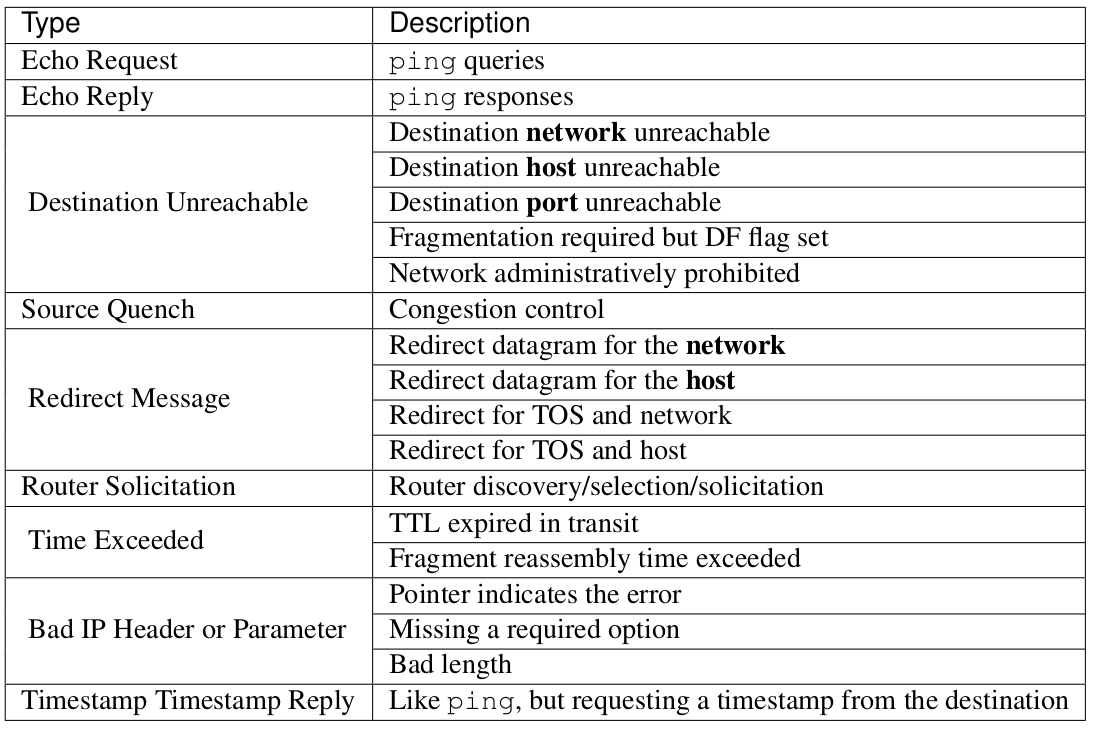
\includegraphics{img/ICMP_types.png}
\item
  The Echo and Timestamp formats are queries, sent by one host to
  another.
\item
  Most of them are all error messages, sent by a router to the sender of
  the offending packet.

  \begin{itemize}
  \tightlist
  \item
    Error-message formats contain the IP header and next 8 bytes of the
    packet in question; the 8 bytes will contain the TCP or UDP port
    numbers.
  \item
    Redirect and Router Solicitation messages are informational, but
    follow the error-message format.
  \item
    Query formats contain a 16-bit Query Identifier, assigned by the
    query sender and echoed back by the query responder.
  \end{itemize}
\end{itemize}

    \section{Routing-Update Algorithms}\label{routing-update-algorithms}

    \subsection{Distance-Vector Routing-Update
Algorithm}\label{distance-vector-routing-update-algorithm}

\begin{itemize}
\tightlist
\item
  Distance-vector is the simplest routing-update algorithm used by the
  Routing Information Protocol

  \begin{itemize}
  \tightlist
  \item
    Routers identify their router neighbors and add a thrid column to
    their forwarding tables representing the total \textbf{cost} for
    delivery to the corresponding destination

    \begin{itemize}
    \tightlist
    \item
      Through some sort of neighbor-discovery mechanism
    \item
      The cost are the distance
    \end{itemize}
  \item
    Forwarding table entries are of the form \(\langle\)destination,
    next\_hop, cost\(\rangle\)
  \item
    Cost are administratively assigned to each link
  \item
    The algorithm calculates the total cost as the sum of the link cost
    along the path

    \begin{itemize}
    \tightlist
    \item
      If a cost of 1 is assigned to each link it is called the hopcount
      metric
    \item
      Link cost can also reflect each linkøs bandwidth, or delay
    \end{itemize}
  \item
    Each router reports the \(\langle\)destination, cost\(\rangle\)
    portion of its table to its neighboring router at regular intervals

    \begin{itemize}
    \tightlist
    \item
      These table portions are the vectors
    \end{itemize}
  \item
    Each router monitors its continued connectivity to each neighbor

    \begin{itemize}
    \tightlist
    \item
      If a neighbor becomes unreachable its reachability cost is set to
      infinity
    \end{itemize}
  \end{itemize}
\end{itemize}

    \subsubsection{Update rules}\label{update-rules}

\begin{itemize}
\tightlist
\item
  Let \(A\) be a router receiving a report \(\langle D, c_D \rangle\)
  from neighbor \(N\) at cost \(c_N\), this means that \(A\) can reach
  \(D\) via \(N\) with cost \(c=c_D+c_N\). \(A\) updates its own table
  according to these rules

  \begin{enumerate}
  \def\labelenumi{\arabic{enumi}.}
  \tightlist
  \item
    \textbf{New destination}: D is previously unknown destination. \(A\)
    adds \(\langle D. M, c \rangle\) to its forwarding table
  \item
    \textbf{Lower cost}: D is a known destination with entry
    \(\langle D,M,c_{old} \rangle\). but the new total cost \(c\) is
    less than \(c_{old}\).\(A\) switches to the cheaper route, updating
    its entry for D to \(\langle D,N,c \rangle\)

    \begin{itemize}
    \tightlist
    \item
      It is possible that \(M=N\)
    \item
      If \(c=c_{old}\) A ignores the new report
    \end{itemize}
  \item
    \textbf{Mext\_hop increase:} \(A\) has an existing
    \(\langle D,N,c_{old} \rangle\) and the new total cost \(c\) is
    greater than \(c_{old}\) . \(A\) updates its entry for \(D\) to
    \(\langle D,N,c \rangle\)
  \end{enumerate}
\end{itemize}

    \subsection{Distance-Vector Slow-Convergence
Problem}\label{distance-vector-slow-convergence-problem}

\begin{itemize}
\tightlist
\item
  The \textbf{Distance-Vector Slow-Convergence Problem} happens when a
  link breaks and another neighbors sends a packets before the link
  where the it broken

  \begin{itemize}
  \tightlist
  \item
    Results in an infinite loop since the to neighbors sends the packet
    to each other for ever
  \end{itemize}
\item
  Fixes to the Distance Vector Slow-Convergence Problem

  \begin{itemize}
  \tightlist
  \item
    The simplest fix to this problem is to use a small value for
    infinity

    \begin{itemize}
    \tightlist
    \item
      No path can be longer than this value
    \end{itemize}
  \item
    Under \textbf{split horizon} if \(A\) uses \(N\) as its next\_hop
    for destination \(D\) then \(A\) simply does not report to \(N\)
    that it can reach \(D\)

    \begin{itemize}
    \tightlist
    \item
      When preparing a report to \(N\) it first deletes all entries that
      have \(N\) as next\_hop
    \item
      Can prevent all linear routing loops but cannot prevent all non
      linear
    \item
      Can also use \textbf{poison reverse} where a cost of \(\infty\) is
      report instead of deleting them
    \end{itemize}
  \item
    Under \textbf{Triggered Updates} any router should report
    immediately to its neighbors whenever it detects any change for the
    worse
  \item
    \textbf{Hold down} dictates that the receiver does not use new
    alternative routes for a period of time following the discovery of
    unreachability

    \begin{itemize}
    \tightlist
    \item
      This gives time for the bad news to arrive
    \end{itemize}
  \end{itemize}
\end{itemize}

    \section{Abstract sliding windows}\label{abstract-sliding-windows}

    \subsection{Building Reliable Transport:
Stop-and-Wait}\label{building-reliable-transport-stop-and-wait}

\begin{itemize}
\tightlist
\item
  \texttt{Data{[}N{]}jj} represents the Nth data packes

  \begin{itemize}
  \tightlist
  \item
    is acknowledge by \texttt{ACK{[}N{]}}
  \end{itemize}
\item
  In the \textbf{stop-and-wait} version of retransmit-on-timeout, the
  sender sends only one outstanding packet at a time

  \begin{itemize}
  \tightlist
  \item
    If there is no response the packet may be retransmitted
  \item
    The sender does not send \texttt{Data{[}N+1{]}} until it has
    received \texttt{ACK{[}N{]}}
  \item
    Each side has only one packet in play at a time
  \item
    If the \texttt{ACK{[}N{]}} is lost the sender sends a duplicate
    \texttt{Data{[}N{]}} and the receiver has implemented a
    \textbf{retransmit-on-duplicate}
  \item
    Each site must implement a \textbf{retransmit-on-timeout}

    \begin{itemize}
    \tightlist
    \item
      Otherwise a lost packet leads to a deadlock
    \end{itemize}
  \item
    The receiver must either implement retransmit-on-timeout or
    \textbf{retransmit-on-duplicate}
  \item
    To avoid the \textbf{Sorcerer's Apprentice Bug} were the double
    amount of packages is send only one side should only implement one
    strategy

    \begin{itemize}
    \tightlist
    \item
      Usually the sender only implements the
      \textbf{retransmit-on-timeout}
    \end{itemize}
  \end{itemize}
\item
  Stop-and-wait provides a simple form of \textbf{flow control} to
  prevent data from arriving at the receiver faster than it can be
  handled

  \begin{itemize}
  \tightlist
  \item
    The stop-and-wait mechanism will prevent data from arriving too fast
    if the time to process a received package is less than one RTT
  \item
    If the processing time is slightly larger than RTT, all the receiver
    has to do is wait to send \texttt{ACK{[}N{]}} until
    \texttt{Data{[}N{]}} not only has arrived but also been processed
    and the receiver is ready
  \item
    To show that data has been received but the receiver is has not
    processed it yet the \texttt{ACK}\(_{\text{WAIT}}\){[}N{]} is used
    and when ready the ACK\(_\text{GO}\){[}N{]} is used

    \begin{itemize}
    \tightlist
    \item
      Creates a new problem where the sender is waiting for the
      ACK\(_\text{GO}\){[}N{]} but it is lost, which can be solved by
      the receiver using the retransmit-on-timeout in that period.
    \end{itemize}
  \end{itemize}
\end{itemize}

    \subsection{Sliding Windows}\label{sliding-windows}

\begin{itemize}
\tightlist
\item
  Sliding Windows want to improve on the efficiency of stop and wait by
  allowing the sender to send multiple packages at once

  \begin{itemize}
  \tightlist
  \item
    \texttt{ACK{[}N{]}} cannot be sent until \texttt{Data{[}K{]}} has
    arrived for all \(K \leq N\)
  \item
    The sender picks a \textbf{window size}, winsize, which is the
    amount of packets the sender is allowed to send before waiting for
    an \texttt{ACK}

    \begin{itemize}
    \tightlist
    \item
      The sender keeps a state variable \textbf{last\_ACKed} which
      represents the last packets which it has received an ACK from the
      other end (initially 0 if packets are one indexed)
    \end{itemize}
  \item
    At any instant, the sender may send packets numbered last\_ACKed +1
    through last\_ACKed+winsize

    \begin{itemize}
    \tightlist
    \item
      This range is known as the \textbf{window}
    \end{itemize}
  \item
    If \texttt{ACK{[}N{]}} arrives with N\textgreater{}last\_ACKed, the
    windows slides forward

    \begin{itemize}
    \tightlist
    \item
      We set lasst\_ACKed = N
    \end{itemize}
  \item
    If there is no packet reordering and no packets losses the windows
    will slides forward in one units at a time
  \end{itemize}
\item
  The bandwidth \(\times\) RTT product is generally the optimum value
  for the window size

  \begin{itemize}
  \tightlist
  \item
    If the sender chooses a winsize larger than this, the RTT grows due
    to queuing delays
  \item
    The sender is often more interested in bandwidth
    RTT\(_\text{noLoad}\)

    \begin{itemize}
    \tightlist
    \item
      Sometimes referred to as the \textbf{transit capacity} of the
      route
    \item
      A window size smaller than this means underutilization of the
      network
    \end{itemize}
  \end{itemize}
\item
  Sliding windows can work pretty well with the receiver assuming
  winsize=1

  \begin{itemize}
  \tightlist
  \item
    Like the sender, the receiver will also maintain the state variable
    last\_ACKede
  \item
    At any instant the receiver is ready to receive
    Data{[}last\_ACKed+1{]} through Data{[}last\_ACKed+winsize{]}.
  \end{itemize}
\item
  If no response is received the sender only sends the first lost
  package

  \begin{itemize}
  \tightlist
  \item
    When a full timeout has occurred the sliding windows process has to
    ground in a halt, which is called \textbf{pipeline drain}
  \end{itemize}
\end{itemize}

    \section{UDP}\label{udp}

\begin{itemize}
\tightlist
\item
  UDP header 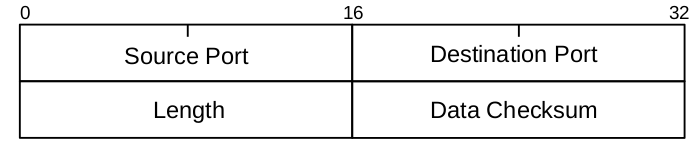
\includegraphics{img/udp_header.png}
\item
  UDP is fairly basic

  \begin{itemize}
  \tightlist
  \item
    The two features it adds beyond IP are \textbf{port numbers} and a
    \textbf{checksum}
  \item
    The port numbers are what makes UDP into a real transport protocol
    with them a process can not connect as an individual server process

    \begin{itemize}
    \tightlist
    \item
      Rather than simply a host
    \end{itemize}
  \item
    UDP is unreliable in that there is no UDP-layer attempt at timeouts
    timeouts, acknowledgment and retransmission

    \begin{itemize}
    \tightlist
    \item
      Applications written for UDP must implement these
    \end{itemize}
  \item
    As with TCP, a UDP pair \(\langle\)host,port\(\rangle\) is known as
    a socket
  \item
    UDP is \textbf{unconnected} or \textbf{stateless}

    \begin{itemize}
    \tightlist
    \item
      If an application has opened a port on a host, any other host on
      the Internet may deliver packets to that
      \(\langle\)host,port\(\rangle\) socket without preliminary
      negotiation.
    \end{itemize}
  \item
    UDP packets use a 16-bit Internet \textbf{checksum} on the data

    \begin{itemize}
    \tightlist
    \item
      Can be disabled and set to an all 0-bits value
    \item
      It covers the UDP header, the UDP data and also a \emph{"pseudo-IP
      header"} that includes the source and destination IP addresses.
    \item
      If a NAT router rewrites an IP address or port the checksum must
      be updated
    \end{itemize}
  \item
    UDP packets can be dropped due to queue overflows either at an
    intervening route or at the receiving host
  \item
    UDP is popular for local transport

    \begin{itemize}
    \tightlist
    \item
      Is typically used as a transport basis for RPC
    \end{itemize}
  \item
    UDP is well suited for \emph{"request-reply"} sematics

    \begin{itemize}
    \tightlist
    \item
      Uses less overhead than TCP
    \end{itemize}
  \item
    UDP is popular for \textbf{real-time} transport

    \begin{itemize}
    \tightlist
    \item
      Because of the \textbf{loss tolerance}
    \item
      RTP is built on top of UDP rather than TCP (common for VoIP calls)
    \end{itemize}
  \end{itemize}
\end{itemize}

    \subsection{Trivial File Transport Protocol
(TFTP)}\label{trivial-file-transport-protocol-tftp}

\begin{itemize}
\tightlist
\item
  TFTP supports file transfers in both directions

  \begin{itemize}
  \tightlist
  \item
    Does not support a mechanism for authentication
  \item
    Uses stop-and-wait and often a fixed timeout interval
  \item
    Typically confined to internal use within a LAN
  \end{itemize}
\item
  TFTP has five packet types

  \begin{itemize}
  \tightlist
  \item
    Read ReQuest, RRQ containing the filename and a text/binary
    indication
  \item
    Write Request, WRQ
  \item
    Data, containing a 16-bit clock number and up to 512 bytes of data
  \item
    ACK, containing a 16-bit block number
  \item
    Error, for certain designated errors

    \begin{itemize}
    \tightlist
    \item
      All errors other than "Unknown Transfer ID" are cause for sender
      termination
    \end{itemize}
  \end{itemize}
\item
  Data block numbering begins at 1

  \begin{itemize}
  \tightlist
  \item
    The packet with the Nth block of data is denoted as Data{[}N{]} and
    acknowledgements are Ack{[}N{]}
  \item
    All blocks o data contain 512 bytes except the final block

    \begin{itemize}
    \tightlist
    \item
      The final block is identified by containing less than 512 bytes of
      data
    \item
      If the file size was divisible by 512, the final block will
      contain 0 bytes of data
    \end{itemize}
  \item
    TFTP numbers are 16 bits in length, and are not allowed to wrap
    around
  \end{itemize}
\item
  The TFTP server listens on UDP port 69 for arriving RRQ packets

  \begin{itemize}
  \tightlist
  \item
    For each RRQ requesting a valid file, TFTP server implementations
    almost always create a separate process (or thread) to handle the
    transfer

    \begin{itemize}
    \tightlist
    \item
      That child process will obtain an entirely new UDP port, which
      will be used for all further interaction with the client for this
      particular transfer
    \end{itemize}
  \end{itemize}
\item
  In the absence of packet loss or other errors, TFTP file requests
  typically proceed as follows:

  \begin{enumerate}
  \def\labelenumi{\arabic{enumi}.}
  \tightlist
  \item
    The client sends a RRQ to server port 69.
  \item
    The server creates a child process, which obtains a new port,
    s\_port, from the operating system.
  \item
    The server child process sends Data{[}1{]} from s\_port.

    \begin{itemize}
    \tightlist
    \item
      Refered to as \textbf{latching on} to that port
    \end{itemize}
  \item
    The client receives Data{[}1{]}, and thus learns the value of
    s\_port. The client will verify that each future Data{[}N{]} arrives
    from this same port.
  \item
    The client sends ACK{[}1{]} (and all future ACKs) to the server's
    s\_port.
  \item
    The server child process sends Data{[}2{]}, etc, each time waiting
    for the client ACK{[}N{]} before sending Data{[}N+1{]}.
  \item
    The transfer process stops when the server sends its final block, of
    size less than 512 bytes, and the client sends the corresponding
    ACK.
  \end{enumerate}
\end{itemize}

    \subsection{Fundamental Transport}\label{fundamental-transport}

    \subsection{Fundamental Transport
Issues}\label{fundamental-transport-issues}

\begin{itemize}
\tightlist
\item
  Some issues regarding any transport strategy

  \begin{itemize}
  \tightlist
  \item
    Old Duplicate Packets

    \begin{itemize}
    \tightlist
    \item
      Happens when a package is lost due to delay, a duplicate one is
      send and then a new connection mistakes it
    \item
      A packet from a previous instance of the connection is called an
      \textbf{external} old duplicate

      \begin{itemize}
      \tightlist
      \item
        Two separate instances of a connection between the same socket
        addresses are sometimes known as \textbf{incarnations} of the
        connection, particularly in the context of TCP.
      \item
        The TFTP defense to this is that both endpoints try and choose a
        different port for each separate transfer
      \end{itemize}
    \item
      \textbf{Internal} old duplicate could happen if the data numbers
      was allowed to wrap around
    \end{itemize}
  \item
    Lost Final ACK

    \begin{itemize}
    \tightlist
    \item
      One cannot be certain that the final ACK is received because no
      ack is send to the receiver
    \item
      It is addressed by TFTP by recommending that the receiver enter
      into a \textbf{DALLY} state when it has to sent the final ACK

      \begin{itemize}
      \tightlist
      \item
        In this state the receiver responds only to deuplicates of the
        final DATA packet and retransmit the final ACK
      \item
        The dally state will expire after an interval which should be at
        least twicer the senders timeout interval
      \item
        Reduces greatly the possibility of the last ACK being lost
      \end{itemize}
    \end{itemize}
  \item
    Duplicated Connection Request

    \begin{itemize}
    \tightlist
    \item
      It happens when a connection cancels a read transfers and starts
      another one

      \begin{itemize}
      \tightlist
      \item
        Then the new transfer can get the old once packets by mistake
      \end{itemize}
    \item
      It can be solved by the receiver changing port number
    \end{itemize}
  \item
    Reboot

    \begin{itemize}
    \tightlist
    \item
      TFTP has to take into account that one side may reboot between
      messages from the other side
    \item
      It is problem with huge importance
    \end{itemize}
  \end{itemize}
\end{itemize}

    \section{TCP}\label{tcp}

\begin{itemize}
\tightlist
\item
  The \textbf{End-to-End} Principle states that transport issues are the
  responsibility of the endpoints in questions
\item
  The TCP header: 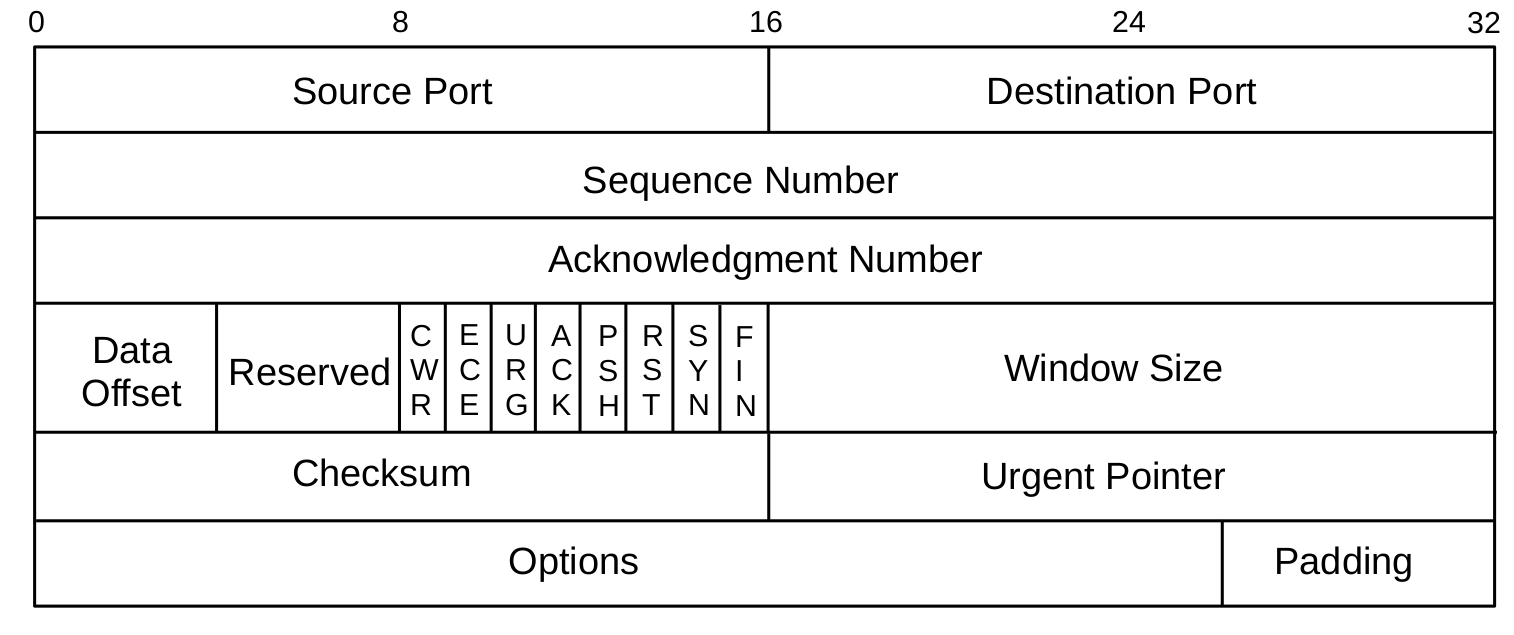
\includegraphics{img/tcp_header.png}

  \begin{itemize}
  \tightlist
  \item
    The checksum covers the TCP header, the TCP data and an IP "pseudo
    header" the includes the source and destination IP addresses

    \begin{itemize}
    \tightlist
    \item
      Must be updated by a NAT router that modifies any header values
    \end{itemize}
  \item
    The \textbf{sequence} and \textbf{acknowledgement} numbers are for
    numbering the data at the byte level

    \begin{itemize}
    \tightlist
    \item
      This allows TCP to send 1024 blocks of data incrementing the
      sequence number by 1024 between successive packets or send 1-byte
      telnet packets, incrementing the sequence number by 1 each time
    \item
      There is no distinction between DATA and ACK packets

      \begin{itemize}
      \tightlist
      \item
        All packets carrying data from A to B also carry the most
        current acknowledgement of data sent from B to A.
      \item
        Many TCP applications are largely unidirectional
      \end{itemize}
    \item
      It is traditional to refer to the data portion of TCP packets as
      \textbf{segments}
    \item
      The value of the sequence number is the position of the first byte
      of the packet in the data stream or the position of where the
      first byte would be in case no data was sent
    \item
      The value of the acknowledgment number represents the byte
      position for the next byte expected
    \item
      The sequence and acknowledgment numbers, as sent, represent these
      relative values plus an Initial Sequence Number, or ISN, that is
      fixed for the lifetime of the connection.

      \begin{itemize}
      \tightlist
      \item
        Each direction of a connection has its own ISN
      \end{itemize}
    \item
      The TCP acknowledgements are \textbf{cumulative}

      \begin{itemize}
      \tightlist
      \item
        It acknowledging receipt of all data byte numbered less than N
        where N is the acknowledgment number
      \end{itemize}
    \end{itemize}
  \item
    The TCP header defines the following flag bits

    \begin{itemize}
    \tightlist
    \item
      \textbf{SYN}: for SYNchronize, marks packets that are part of the
      new connection handshake
    \item
      \textbf{ACK}: indicates that the header ACcknowledgment field is
      valid, that is all but the first packet
    \item
      \textbf{FIN}: for FINish, marks packets involved in the connection
      closing
    \item
      \textbf{PSH}: for PuSH, marks \emph{"non-full"} packets that
      should be delivered promptly at the far end
    \item
      \textbf{RST}: for ReSet, indicates various error conditions
    \item
      \textbf{URG}: for URGent, part of a now-seldom-used mechanism for
      high-priority data
    \item
      \textbf{CWR} and \textbf{ECE}: part of the Explicit Congestion
      Notification mechanism
    \end{itemize}
  \end{itemize}
\end{itemize}

    \subsection{TCP Connection
Establishment}\label{tcp-connection-establishment}

\begin{itemize}
\tightlist
\item
  TCP connections are established via an exchange known as the
  \textbf{three-way handshake}, A is the client and B is the LISTENing
  server then the handshake goes as follows

  \begin{itemize}
  \tightlist
  \item
    A sends B a packet with the SYN bit set (a SYN packet)
  \item
    B responds with a SYN packet of its own, the ACK bit is now also set
  \item
    A responds to B's SYN with its own ACK
  \end{itemize}
\item
  Normally a three way handshake is triggered by an application's
  request to connect

  \begin{itemize}
  \tightlist
  \item
    Data can only be send after the handshake completes
  \item
    It is vulnerable to an attack known as \textbf{SYN flooding}

    \begin{itemize}
    \tightlist
    \item
      The attacker sends a large number of SYN packets to a server B
    \item
      For each arriving resource B must allocate resources and B's
      resources may face exhaustion
    \end{itemize}
  \end{itemize}
\item
  To \textbf{close} the connection, a superficially similar exchange
  involving FIN packets may occur

  \begin{itemize}
  \tightlist
  \item
    A sends B a packet with the FIN bit set (a FIN packet), announcing
    that it has finished sending data
  \item
    B sends A an ACK of the FIN
  \item
    B may continue to send additional data to A
  \item
    When B is also ready to cease sending, it sends its own FIN to A
  \item
    A sends B an ACK of the FIN; this is the final packet in the
    exchange
  \end{itemize}
\item
  When closing a connection it is important to use \texttt{shutdown}
  instead of \texttt{close}

  \begin{itemize}
  \tightlist
  \item
    \texttt{close} just closes the connection and does not listen for
    further data
  \item
    If the non closed part tries to send data the closed one might send
    a \texttt{rst} which means that all data sent is lost
  \end{itemize}
\end{itemize}

    \subsection{TIMEWAIT}\label{timewait}

\begin{itemize}
\tightlist
\item
  The TIMEWAIT state is entered by whichever side initiates the
  connection close

  \begin{itemize}
  \tightlist
  \item
    In the event of a simultaneous close both sides enter TIMEWAIT
  \item
    It is to last for a time \(2 \ \times\) MSL

    \begin{itemize}
    \tightlist
    \item
      MSL is an agreed-upon value for the maximum lifetime on the
      Internet of an IP packet
    \item
      Traditionally 60 seconds but modern 30 seconds
    \end{itemize}
  \item
    One function is to solve the external-old-duplicates problem

    \begin{itemize}
    \tightlist
    \item
      Requires that enough time has passed for old duplicates to
      disappear
    \end{itemize}
  \item
    A second function of TIMEWAIT is to address the lost-final-ACK
    problem

    \begin{itemize}
    \tightlist
    \item
      TIMEWAIT only blocks reconnections for which both sides reuse the
      same port they used beforej
    \end{itemize}
  \end{itemize}
\end{itemize}

    \subsection{TCP state diagram}\label{tcp-state-diagram}

\begin{itemize}
\tightlist
\item
  The following is a \textbf{state diagram} for TCP
  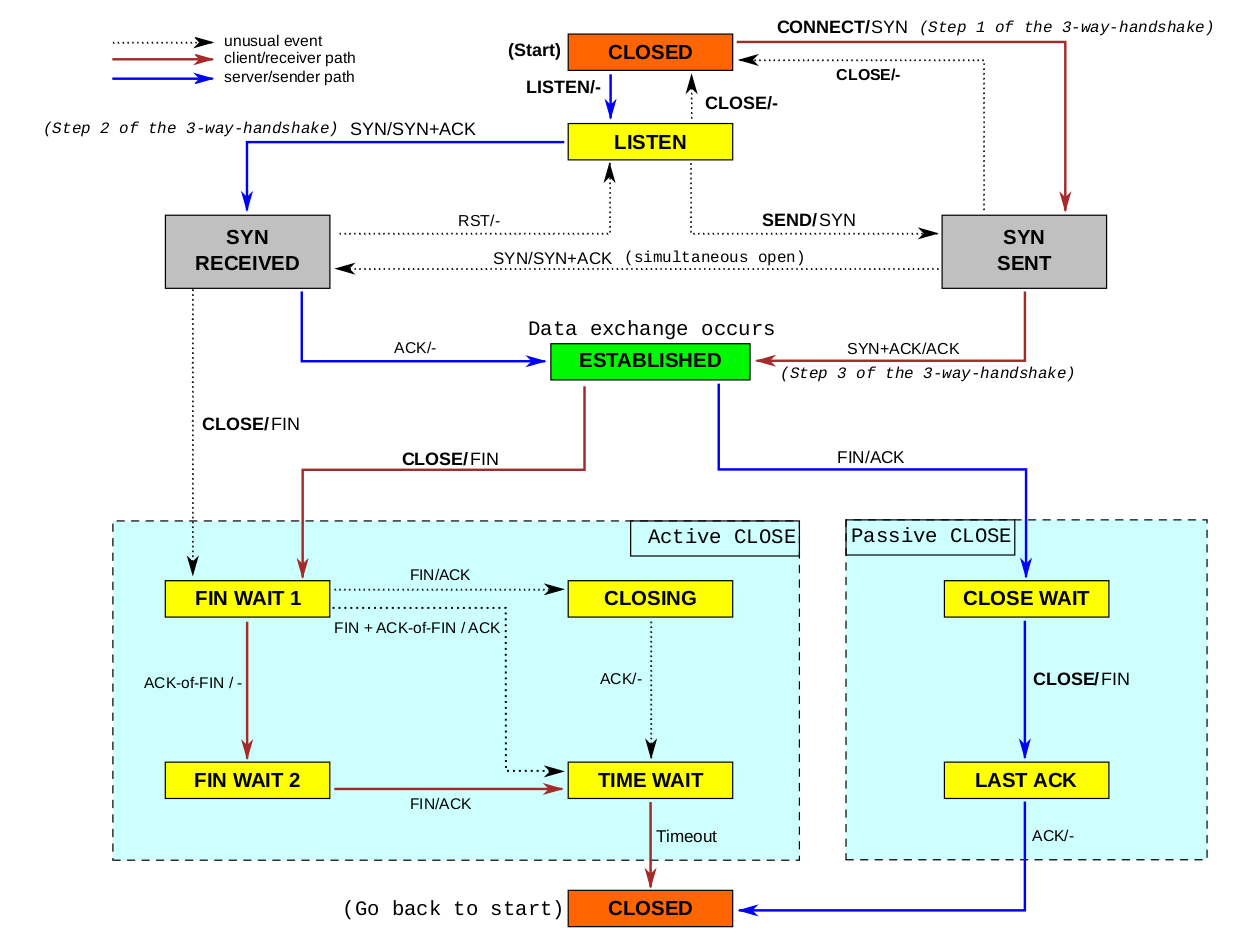
\includegraphics{img/tcp_state.png}

  \begin{itemize}
  \tightlist
  \item
    The blue arrows indicate the sequence of state transitions typically
    followed by the server
  \item
    The brown arrows represent the client
  \item
    Arrows are labeled with \textbf{event/action}
  \item
    The ESTABLISHED state and the states below it are sometimes called
    the \textbf{synchronized} states

    \begin{itemize}
    \tightlist
    \item
      Since both sides have confirmed each others ISN values
    \end{itemize}
  \end{itemize}
\end{itemize}

    \section{The Web and HTTP}\label{the-web-and-http}

\begin{itemize}
\tightlist
\item
  A webpage consists of \textbf{objects}

  \begin{itemize}
  \tightlist
  \item
    A \textbf{object} is a file
  \end{itemize}
\item
  HTTP uses TCP as its underlying transport protocol

  \begin{itemize}
  \tightlist
  \item
    The HTTP client first initiates a TCP connection
  \item
    The client sends HTTP request messages into its socket interface and
    receives HTTP response messages from its socket interface.
  \item
    The server receives request messages from its socket interface and
  \item
    HTTP is said to a \textbf{stateless} protocols because thea server
    does not store and state on the different clients
  \end{itemize}
\item
  A \textbf{non-persistent connection} is where each request/response
  pair is send over separate TCP connections
\item
  A \textbf{persistent connection} is where each request/response pair
  is send over the same TCP connection

  \begin{itemize}
  \tightlist
  \item
    Used by the default mode in HTTP
  \end{itemize}
\end{itemize}

    \subsection{HTTP request message
format}\label{http-request-message-format}

\begin{itemize}
\item
  There are two different types of HTTP messages, request messages and
  response messages
\item
  Example of a typical HTTP request message

\begin{verbatim}
GET /somedir/page.html HTTP/1.1
Host: www.someschool.edu
Connection: close
User-agent: Mozilla/5.0
Accept-language: fr
\end{verbatim}

  \begin{itemize}
  \tightlist
  \item
    The first line of an HTTP request message is called the
    \textbf{request line}

    \begin{itemize}
    \tightlist
    \item
      It has three fields: the message field, the URL field and HTTP
      version field
    \item
      The \texttt{HEAD} method is the same as the \texttt{GET} but it
      leaves out the body
    \end{itemize}
  \item
    The subsequent lines are called \textbf{header lines}

    \begin{itemize}
    \tightlist
    \item
      The header line starting with \texttt{Host:} specifies where the
      host lives
    \item
      By supplying the \texttt{Connection:\ close} the client tells the
      server that it doesn't want to bother with a persistent connection
    \item
      The \texttt{User-agent:} line what browser type is making the
      request
    \item
      The \texttt{Accept-language:} tells the server that it want the
      french version of the site
    \end{itemize}
  \end{itemize}
\end{itemize}

\begin{figure}
\centering
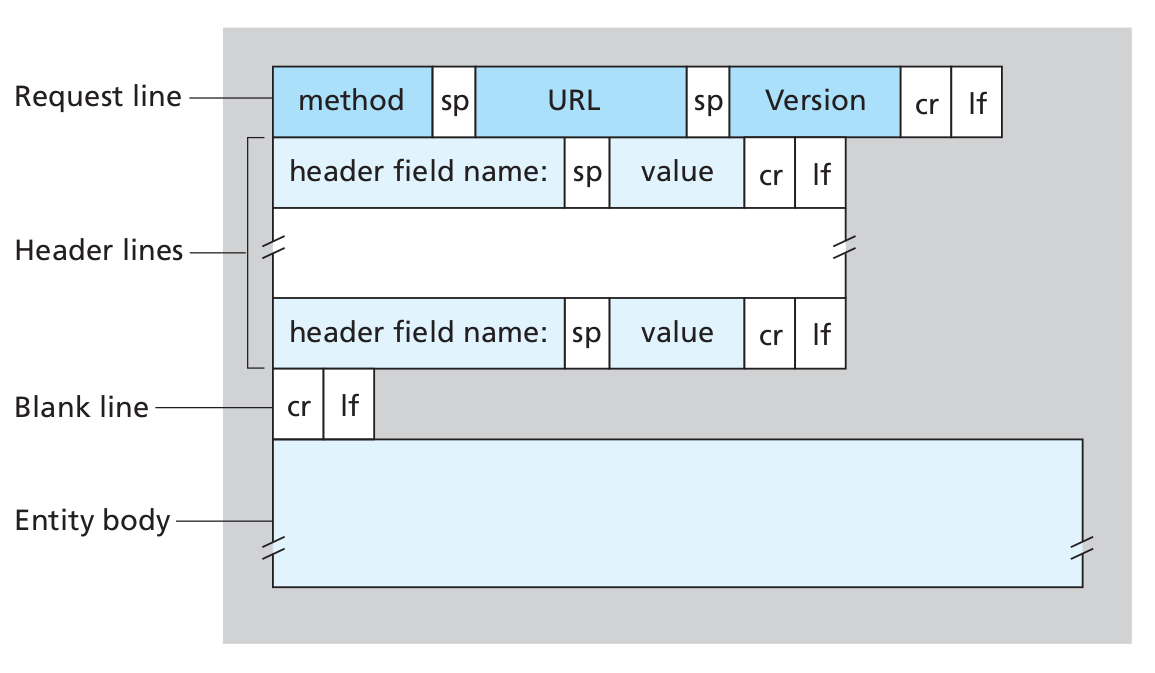
\includegraphics{img/http_request_header_format.png}
\caption{http\_request\_header\_format}
\end{figure}

    \subsection{HTTP Response Message}\label{http-response-message}

\begin{itemize}
\item
  Example of HTTP response message

\begin{verbatim}
HTTP/1.1 200 OK
Connection: close
Date: Tue, 09 Aug 2011 15:44:04 GMT
Server: Apache/2.2.3 (CentOS)
Last-Modified: Tue, 09 Aug 2011 15:11:03 GMT
Content-Length: 6821
Content-Type: text/html

(data data....)
\end{verbatim}

  \begin{itemize}
  \tightlist
  \item
    The first line is the status line which has three fields: the
    protocol version, the status code and the corresponding status
    message
  \item
    The other lines before the data is the header lines
  \item
    The \texttt{Connection:\ close} tells the client that it is going to
    close the connection after sending this message
  \item
    The \texttt{Date:} tells the client which and date the HTTP response
    message was created
  \item
    The \texttt{Server:} indicates which server has created the message
  \item
    The \texttt{Last-Modified:} indicates the time or date the object
    was created or modified
  \item
    The \texttt{Content-Length:} indicates the number of bytes being
    sent
  \item
    The \texttt{Content-Type:} indicates the objects type
  \end{itemize}
\end{itemize}

\begin{figure}
\centering
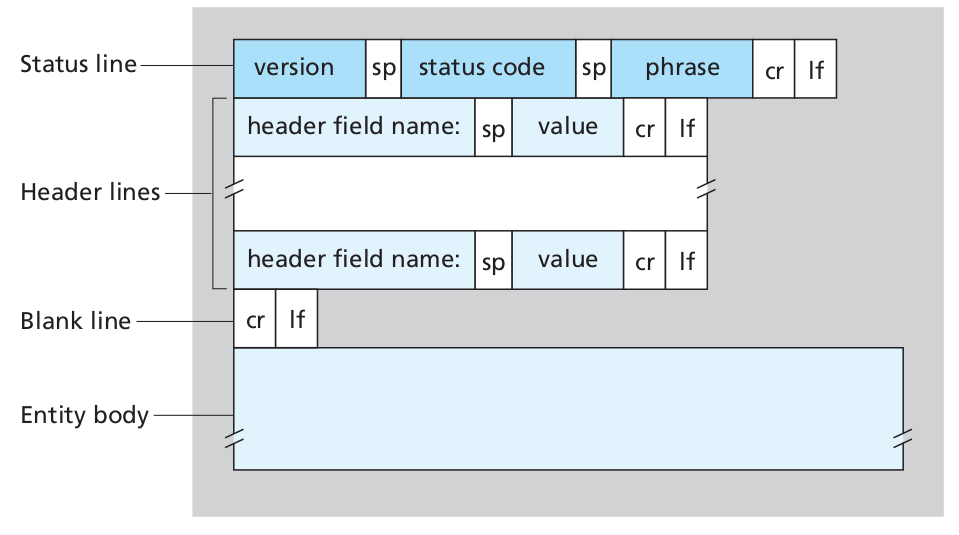
\includegraphics{img/http_response_header_format.png}
\caption{http\_response\_header\_format}
\end{figure}

    \subsection{Cookies}\label{cookies}

\begin{itemize}
\tightlist
\item
  Cookies allows sites to keep track of users
\item
  Example of a cookie header line when a new cookie is made:
  \texttt{Set-cookie:\ 1678}
\item
  Example of a cookie in a normal request: \texttt{Cookie:\ 1678}
\item
  A cookie consists of three components

  \begin{enumerate}
  \def\labelenumi{\arabic{enumi}.}
  \tightlist
  \item
    A cookie header line in the HTTP response message
  \item
    A cookie header line in the HTTP request message
  \item
    A cookie file kept on the user's end system and managed by the
    user's browser
  \item
    A back-end database at the Web site.
  \end{enumerate}
\end{itemize}

    \subsection{Web-caching}\label{web-caching}

\begin{itemize}
\tightlist
\item
  A Web cache also called a proxy server is a network entity that
  satisfies HTTP requests on the behalf of an origin Web server.

  \begin{itemize}
  \tightlist
  \item
    It has its own disk storage and keeps copies of recently requested
    objects in this storage.
  \end{itemize}
\item
  The browser interacts with the net-cache in the following way

  \begin{enumerate}
  \def\labelenumi{\arabic{enumi}.}
  \tightlist
  \item
    The browser establishes a TCP connection to the Web cache and sends
    an HTTP request for the object to the Web cache.
  \item
    The Web cache checks to see if it has a copy of the object stored
    locally.

    \begin{itemize}
    \tightlist
    \item
      If it does, the Web cache returns the object within an HTTP
      response message to the client browser.
    \end{itemize}
  \item
    If the Web cache does not have the object, the Web cache opens a TCP
    connection to the origin server. The Web cache then sends an HTTP
    request for the object into the cache-to-server TCP connection.

    \begin{itemize}
    \tightlist
    \item
      After receiving this request, the origin server sends the object
      within an HTTP response to the Web cache.
    \end{itemize}
  \item
    When the Web cache receives the object, it stores a copy in its
    local storage and sends a copy, within an HTTP response message, to
    the client browser

    \begin{itemize}
    \tightlist
    \item
      This is done over the existing TCP connection between the client
      browser and the Web cache.
    \end{itemize}
  \end{enumerate}
\item
  A web cache is typically purchased and installed by an ISP
\item
  At web cache can substantually reduce an institution's access link to
  the Internet.
\end{itemize}

    \subsection{The conditional GET}\label{the-conditional-get}

\begin{itemize}
\tightlist
\item
  The mechanism \textbf{conditional GET} allows the web cache to verify
  that the objects are up to date
\item
  An HTTP request is a conditional GET if

  \begin{enumerate}
  \def\labelenumi{\arabic{enumi}.}
  \tightlist
  \item
    The request message uses the GET message
  \item
    The request message includes an \texttt{If-Modified-Since:} header
    line.
  \end{enumerate}
\end{itemize}

    \section{FTP}\label{ftp}

\begin{itemize}
\tightlist
\item
  FTP is used to transfer files from a remote system to another system

  \begin{itemize}
  \tightlist
  \item
    The user first provides the host name of the remote host

    \begin{itemize}
    \tightlist
    \item
      This causes the FTP client to establish an TCP connection with the
      FTP server process on the remote host
    \end{itemize}
  \item
    The users then provides the user identification and password

    \begin{itemize}
    \tightlist
    \item
      This is send over TCP as a part of the FTP commands
    \end{itemize}
  \item
    Once the server has authorized the user, the user copies one or more
    files stored in the local file system into the remote file system
    (or vice versa).
  \end{itemize}
\item
  FTP uses two parallel connection for to transfer a file a
  \textbf{control connection} and a \textbf{data connection}

  \begin{itemize}
  \tightlist
  \item
    The control connection is used for sending control information
    between the two connections

    \begin{itemize}
    \tightlist
    \item
      Information such as user identification, password, commands to
      change remote directory, and commands to "put" and "get" files.
    \end{itemize}
  \item
    The data connection is used to actually send a file.
  \end{itemize}
\item
  Since FTP uses a separate control connection, FTP is said to send its
  control information \textbf{out-of-band}

  \begin{itemize}
  \tightlist
  \item
    For this reason, HTTP is said to send its control information
    \textbf{in-band}.
  \end{itemize}
\item
  The client side of FTP first initiates a control TCP connection with
  the server side (remote host) on server port number 21.

  \begin{itemize}
  \tightlist
  \item
    The client side of FTP sends the user identification and password
    over this control connection
  \item
    The client also sends commands to change the directory through this
    connection
  \end{itemize}
\item
  When the server side receives a command for a file transfer over the
  control connection, the server side initiates a TCP data connection to
  the client side.

  \begin{itemize}
  \tightlist
  \item
    FTP sends exactly one file over the data connection and then closes
    the data connection.
  \item
    If, during the same session, the user wants to transfer another
    file, the server opens another connection
  \end{itemize}
\item
  Throughout a session FTP maintains a \textbf{state} about each user
\end{itemize}

    \subsection{FTP commands and Replies}\label{ftp-commands-and-replies}

\begin{itemize}
\tightlist
\item
  The commands, from client to server, and replies, from server to
  client, are sent across the control connection in 7-bit ASCII format.
\item
  Common FTP commands

  \begin{itemize}
  \tightlist
  \item
    \texttt{USER\ username}: Used to send user identification to the
    server
  \item
    \texttt{PASS\ password}: Used to send the user password to the
    server
  \item
    \texttt{LIST}: Used to ask the server to send a list of all the
    files in the current directory

    \begin{itemize}
    \tightlist
    \item
      The list of files are send over a new and non-persistent
      data-connection
    \end{itemize}
  \item
    \texttt{RETR\ filename}: Used to retrieve (get) a file from the
    current directory on the remote server
  \item
    \texttt{STOR\ filename}: Used to store (put) a file into the current
    directory on the remote server
  \end{itemize}
\item
  Each command is followed by a corresponding reply from the server to
  the client, which consists of a number with an optional message. Here
  are some examples

  \begin{itemize}
  \tightlist
  \item
    \texttt{331\ Username\ OK,\ password\ required}
  \item
    \texttt{125\ Data\ Data\ connection\ already\ open;\ transfer\ starting}
  \item
    \texttt{425\ Can\textquotesingle{}t\ open\ data\ connection}
  \item
    \texttt{452\ Error\ writing\ file}
  \end{itemize}
\end{itemize}

    \section{Electronic Mail in the
Internet}\label{electronic-mail-in-the-internet}

\begin{itemize}
\tightlist
\item
  Internet mail has three major components: \textbf{user agents},
  \textbf{mail servers} and \textbf{Simple Mail Transfer Protocol
  (SMTP)}
\item
  User agents allow the user to read, reply to, forward, save and
  compose message

  \begin{itemize}
  \tightlist
  \item
    When the user is done composing an email the user agent sends the
    mail to the mail server, where the mail is placed in the mail
    servers outgoing queue
  \end{itemize}
\item
  Mail servers form the core of the e-mail infrastructure.

  \begin{itemize}
  \tightlist
  \item
    Each user has a mailbox located in one of the mail servers
  \item
    Each users mailbox manages and maintains the message that have been
    send to that person
  \item
    A message starts in the sender's user agent, then to the senders
    mail server, and then to the recipient mail server and is then
    deposited in the recipient's mailbox
  \item
    When a user wants to access messages in the mailbox, the mail server
    authenticates the User

    \begin{itemize}
    \tightlist
    \item
      Done using usernames and passwords
    \end{itemize}
  \item
    A mail server must deal with failures in other peoples mail servers
  \item
    If a mail server cannot deliver mail to another mail server it holds
    the message in a message queue and attempts again later

    \begin{itemize}
    \tightlist
    \item
      Is often done every 30 minutes or so
    \item
      If there is no success after several days, the server removes the
      message and notifies the sender with e-mail address
    \end{itemize}
  \end{itemize}
\item
  SMTP is the principal application-layer protocol for Internet
  electronic mail.

  \begin{itemize}
  \tightlist
  \item
    It TCP to transfer mail from the senders mail server to the
    recipient's mail server
  \item
    SMTP has two sides

    \begin{enumerate}
    \def\labelenumi{\arabic{enumi}.}
    \tightlist
    \item
      A client site which executes on the sender's mail server
    \item
      A server side which executes on the recipients mail server
    \end{enumerate}
  \item
    Both the client and the server side run on every mail server
  \item
    When a mail server sends mail to other servers it acts as SMTP
    client
  \item
    When a mail server receives mail from other servers it acts as SMTP
    server
  \end{itemize}
\end{itemize}

    \subsection{SMTP}\label{smtp}

\begin{itemize}
\item
  SMTP restricts the body (not just the headers) of all mail messages to
  simple 7-bit ASCII.
\item
  SMTP does not normally use intermediate mail servers for sending mail,
  instead a direct TCP connection is used
\item
  How SMTP transfers a message from a sending mail server to a receiving
  mail server

  \begin{enumerate}
  \def\labelenumi{\arabic{enumi}.}
  \tightlist
  \item
    The client SMTP has TCP establish a connection to port 25 at the
    server SMTP

    \begin{itemize}
    \tightlist
    \item
      If the server is down the client tries again later
    \end{itemize}
  \item
    The server and client perform some application-layer handshaking

    \begin{itemize}
    \tightlist
    \item
      SMTP clients and servers introduce themselves before transferring
      information
    \item
      The SMTP client indicates the e-mail address of the sender and the
      e-mail of the recipient
    \end{itemize}
  \item
    The client sends the message

    \begin{itemize}
    \tightlist
    \item
      The client repeats this process over the same TCP connection if it
      has other messages to send to the server
    \end{itemize}
  \end{enumerate}
\item
  Example where \texttt{S} is server and \texttt{C} is client

\begin{verbatim}
S: 220 hamburger.edu
C: HELO crepes.fr
S: 250 Hello crepes.fr, pleased to meet you
S: MAIL FROM: <alice@crepes.fr>
S: 250 alice@crepes.fr ... Sender ok
C: RCPT TO: <bob@hamburger.edu>
S: 250 bob@hamburger.edu ... Recipient ok
C: DATA
S: 354 Enter mail, end with "." on a line by itself
C: Do you like ketchup?
C: How about pickles?
C: .
S: 250 Message accepted for delivery
C: QUIT
S: 221 hamburger.edu closing connection
\end{verbatim}

  \begin{itemize}
  \tightlist
  \item
    If more mails are send it begins each new mail with
    \texttt{MAIL\ FROM:\ crepes.fr}
  \end{itemize}
\end{itemize}

    \subsection{SMTP header}\label{smtp-header}

\begin{itemize}
\item
  Example of a SMTP header

\begin{verbatim}
From: alice@crepes.fr
To: bob@hamburger.edu
Subject: Searching for the meaning of life.
\end{verbatim}

  \begin{itemize}
  \tightlist
  \item
    Every header must have a \texttt{FROM} and \texttt{TO} line
  \item
    The \texttt{Subject:} line is optional
  \item
    The header lines are part of the mail message itself
  \end{itemize}
\end{itemize}

    \subsection{Mail Access Protocols}\label{mail-access-protocols}

\begin{itemize}
\item
  SMTP cannot be used to access mails on the server since it uses a push
  operation
\item
  There are a number of popular mail access protocols, including Post
  Office Protocol---Version 3 (POP3), Internet Mail Access Protocol
  (IMAP), and HTTP. 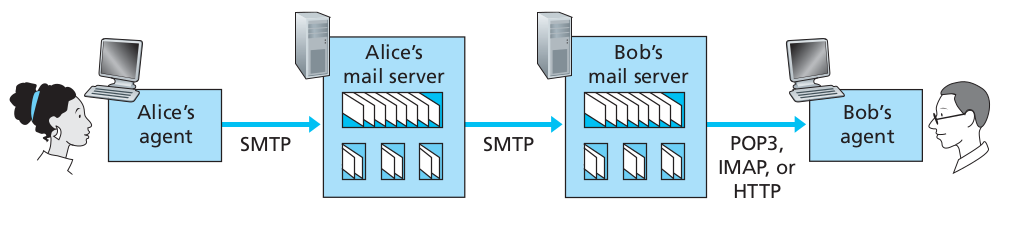
\includegraphics{img/mail_access.png}
\item
  When the client it web based it sends and receives messages from the
  web server using the HTTP protocol
\end{itemize}

    \subsubsection{POP3}\label{pop3}

\begin{itemize}
\item
  POP3 is an extremely simple mail access protocol

  \begin{itemize}
  \tightlist
  \item
    It has limited functionality
  \end{itemize}
\item
  POP3 begins when the user agent open a TCP connection to the mail
  server on port 110
\item
  POP3 progresses through three phases: authorization, transaction, and
  update when a connection has been established

  \begin{itemize}
  \tightlist
  \item
    \textbf{Authorization}: the user agent sends a username and a
    password to authenticate the user
  \item
    \textbf{Transaction}: the user agent retrieves messages and the user
    can

    \begin{itemize}
    \tightlist
    \item
      mark messages for deletion
    \item
      remove deletion marks
    \item
      obtain mail statistics
    \end{itemize}
  \item
    \textbf{Update}: the mail server deletes the messages that were
    marked for deletion

    \begin{itemize}
    \tightlist
    \item
      Occurs after the client has issued the quit command which ends the
      session
    \end{itemize}
  \end{itemize}
\item
  In a POP3 transaction the user agent issues commands and the server
  responds with a reply to each command and there are two possible
  responses

  \begin{itemize}
  \tightlist
  \item
    \texttt{+OK} which indicates that the previous command was fine

    \begin{itemize}
    \tightlist
    \item
      It is sometimes followed by server-to-client data
    \end{itemize}
  \item
    \texttt{-ERR} which indicates that something was wrong with the
    previous command
  \end{itemize}
\item
  The authorization phase has two principal commands

  \begin{itemize}
  \tightlist
  \item
    \texttt{user\ \textless{}username\textgreater{}}
  \item
    \texttt{pass\ \textless{}password\textgreater{}}
  \end{itemize}
\item
  Example of authorization phase on mail server

\begin{verbatim}
telnet mailServer 110
+OK POP3 server ready
user bob
+OK
pass hungry
+OK user successfully logged on
\end{verbatim}
\item
  During the transaction phase the user agent can often be configured to
  \emph{"download and delete"} or \emph{"download and keep"}

  \begin{itemize}
  \tightlist
  \item
    In the download-and-delete mode, the user agent will issue the
    \texttt{list}, \texttt{retr}, and \texttt{dele} commands.

    \begin{itemize}
    \tightlist
    \item
      Since the download-and-delete mode deletes the messages after
      reading them the user will not be able to view them on multiple
      computers
    \end{itemize}
  \item
    In the download-and-keep mode the user agents keeps the messages on
    the server
  \end{itemize}
\item
  Example transtion phase using \emph{download and delete}

\begin{verbatim}
C: list
S: 1 498
S: 2 912
S: .
C: retr 1
S: (blah blah ...
S: .................
S: ..........blah)
S: .
C: dele 1
C: retr 2
S: (blah blah ...
S: .................
S: ..........blah)
S: .
C: dele 2
C: quit
S: +OK POP3 server signing off
\end{verbatim}
\item
  POP3 only maintains the user state during the session
\end{itemize}

    \subsubsection{IMAP}\label{imap}

\begin{itemize}
\tightlist
\item
  It is not possible to maintain a folder hierarchy on a remote server
  using POP3

  \begin{itemize}
  \tightlist
  \item
    This and other problems is solved by the more complex IMAP
  \end{itemize}
\item
  An IMAP server will associated each message with a folder

  \begin{itemize}
  \tightlist
  \item
    When a message first arrives at the server it is associated with the
    recipients INBOX folder
  \item
    The recipient can move a message into a new, user-created folder,
    read the message, delete the message, and so on.
  \end{itemize}
\item
  The IMAP protocol provides commands to allow users to create folders
  move messages from one folder to another

  \begin{itemize}
  \tightlist
  \item
    It also provides commands that allow users to search remote folders
    for messages matching specific criteria
  \end{itemize}
\item
  An IMAP server maintains user state information across IMAP sessions

  \begin{itemize}
  \tightlist
  \item
    Such as the names of folders and which messages are associated with
    which folder
  \end{itemize}
\item
  IMAP has commands that permit the user agent to obtain component of
  messages

  \begin{itemize}
  \tightlist
  \item
    A user can obtain the message header of the message or just one part
    of a multipart MIME message.
  \item
    It is useful for a low-bandwidth connection
  \end{itemize}
\end{itemize}

    \section{DNS}\label{dns}

\begin{itemize}
\tightlist
\item
  The task of DNS is to translate hostnames to IP addresses

  \begin{itemize}
  \tightlist
  \item
    DNS is a distributed database implemented in a hierarchy of DNS
    servers
  \item
    DNS is an application-layer protocol that allows host to query the
    distributed database
  \end{itemize}
\item
  DNS servers are often UNIX machine running the Berkeley Internet Name
  Domain (BIND) software.

  \begin{itemize}
  \tightlist
  \item
    The DNS protocol runs over UDP and uses port 53
  \item
    IT is commonly employed by other application-layer protocols such as
    HTTP, SWTPP, and FTP-to translate hostnames to IP addresses
  \end{itemize}
\item
  DNS call to obtain the IP address of www.someschool.edu example

  \begin{enumerate}
  \def\labelenumi{\arabic{enumi}.}
  \tightlist
  \item
    The same user machine runs the client side of the DNS application.
  \item
    The browser extracts the hostname, www.someschool.edu, from the URL
    and passes the hostname to the client side of the DNS application.
  \item
    The DNS client sends a query containing the hostname to a DNS
    server.
  \item
    The DNS client eventually receives a reply, which includes the IP
    address for the hostname.
  \item
    Once the browser receives the IP address from DNS, it can initiate a
    TCP connection to the HTTP server process located at port 80 at that
    IP address.
  \end{enumerate}
\item
  DNS provides a few other important services in addition to translating
  hostnames to IP addresses:

  \begin{itemize}
  \tightlist
  \item
    \textbf{Host aliasing}: A host with a complicated hostname can have
    one or more alias names.

    \begin{itemize}
    \tightlist
    \item
      The original hostname is said to be the \textbf{canonical
      hostname}
    \end{itemize}
  \item
    \textbf{Mail server aliasing}: DNS can be invoked by a mail
    application to obtain the canonical hostname for a supplied alias
    hostname as well as the IP address of the host.
  \item
    \textbf{Load distribution.} DNS is also used to perform load
    distribution among replicated servers, such as replicated web server

    \begin{itemize}
    \tightlist
    \item
      For replicated servers a set of IP addresses are associated with
      one canonical hostname
    \item
      When clients make a DNS query for a name mapped to a set of
      addresses, the server responds with the entire set of IP
      addresses, but rotates the ordering of the addresses within each
      reply.
    \item
      DNS rotation is also used for e-mail so that multiple mail servers
      can have the same alias name
    \end{itemize}
  \end{itemize}
\end{itemize}

    \subsection{How DNS works}\label{how-dns-works}

\begin{itemize}
\tightlist
\item
  To translate a hostname to an IP address, the application invoke the
  client side of DNS

  \begin{itemize}
  \tightlist
  \item
    It specifies what hostname needs to be translate

    \begin{itemize}
    \tightlist
    \item
      On UNIX it is often the \texttt{getHostName()} function that is
      invoked
    \end{itemize}
  \item
    All DNS query and reply messages are sent within UDP datagrams to
    port 53
  \item
    DNS in the user's host takes over, sending a query message into the
    network.
  \item
    After a delay from milliseconds to seconds DNS in the user's host
    receives a DNS reply message that provides the desired mapping

    \begin{itemize}
    \tightlist
    \item
      This is passed to the invoking application
    \end{itemize}
  \end{itemize}
\item
  In the perspective of the invoking application DNS is a black box
  providing a simple, straightforward translation service

  \begin{itemize}
  \tightlist
  \item
    DNS service is complex, consisting of a large number of DNS servers
    distributed around the globe and an application-layer protocol that
    specifies how the DNS servers and querying host communicate
  \end{itemize}
\item
  Problems with a centralized design simple DNS server includes

  \begin{itemize}
  \tightlist
  \item
    \textbf{A single point of failure}: If the DNS server crashed so
    does the entire Internet
  \item
    \textbf{Traffic volume}: A single DNS server would have to handle
    all DNS queries
  \item
    \textbf{Distant centralized database}: A single DNS server cannot be
    "close to" all the querying clients

    \begin{itemize}
    \tightlist
    \item
      This can lead to significant delays
    \end{itemize}
  \item
    \textbf{Maintenance}: A single DNS server would have to keep records
    for all Internet hosts

    \begin{itemize}
    \tightlist
    \item
      It would not only have to be huge, but also have to be updated
      frequently
    \end{itemize}
  \end{itemize}
\end{itemize}

    \subsubsection{A Distributed, Hierarchical
Database}\label{a-distributed-hierarchical-database}

\begin{itemize}
\tightlist
\item
  DNS uses a large number of servers to deal with the issue of scale

  \begin{itemize}
  \tightlist
  \item
    They are organized in a hierarchical fashion and distributed around
    the world
  \item
    No a single server has all of the mapping for all the servers in the
    world
  \item
    Mappings are distributed across the DNS servers
  \end{itemize}
\item
  There are three classes of DNS servers

  \begin{itemize}
  \tightlist
  \item
    \textbf{Root DNS servers}: There are 13 root DNS servers on the
    internet

    \begin{itemize}
    \tightlist
    \item
      Each server is a network of replicated servers for security and
      reliability purposes
    \end{itemize}
  \item
    \textbf{Top-level-domain (TLD) servers}: These servers are
    responsible for top-level domains such as com, org, net, edu and
    gov, and all of the country top-level domains
  \item
    \textbf{Authoritative DNS servers}: Every organization with publicly
    accessible hosts on the Internet must provide publicly accessible
    DNS records that map the names of those hosts to IP addresses.

    \begin{itemize}
    \tightlist
    \item
      Such as Web servers and mail server
    \item
      An organization's authoritative DNS server houses these DNS
      records
    \item
      An organization can choose to implement its own authoritative DNS
      server to hold these records

      \begin{itemize}
      \tightlist
      \item
        The the organization can pay to have these records stored in an
        authoritative DNS server of some service provider
      \end{itemize}
    \end{itemize}
  \end{itemize}
\item
  A \textbf{local DNS server} does not strictly belong to the the
  hierarchy of servers but is nevertheless central to the DNS
  architecture.

  \begin{itemize}
  \tightlist
  \item
    Each ISP has a local DNS server

    \begin{itemize}
    \tightlist
    \item
      Such as a university, an academic department, an employee's
      company, or a residential ISP
    \item
      Also called a default name server
    \end{itemize}
  \item
    When a host connects to an ISP, the ISP provides the host with the
    IP addresses of one or more of its local DNS servers
  \item
    A host local DNS server is typically "close to" the host

    \begin{itemize}
    \tightlist
    \item
      For an institutional ISP the DNS server may be on the same LAN
    \item
      For a residential ISP it is typically separated from the host by
      no more than a few routers
    \end{itemize}
  \item
    When a host makes a DNS query, the query is sent to the local DNS
    server which acts a proxy

    \begin{itemize}
    \tightlist
    \item
      It forwards the query into the DNS server hierarchy
    \end{itemize}
  \end{itemize}
\item
  A query can be iterative or recursive

  \begin{itemize}
  \tightlist
  \item
    If it is \textbf{iterative}, the Root DNS servers and
    Top-level-domain servers gives the client an IP address of an
    Top-level-domain server and a Autoritative DNS server and it is the
    clients job to contact them
  \item
    If it is \textbf{recursive} the server does all the work contacting
    the correct servers and gives the correct IP address to the client
  \item
    DNS queries to a local DNS server are typically recursive and all
    others are iterative
  \end{itemize}
\end{itemize}

    \subsubsection{DNS caching}\label{dns-caching}

\begin{itemize}
\tightlist
\item
  DNS caching is done each time a DNS server receives a DNS reply

  \begin{itemize}
  \tightlist
  \item
    It can cache the mapping in its local memory
  \item
    If a hostname/IP address pair is cached in a DNS server and another
    query arrives to the same hostname the DNS server can provide the
    desired IP address
  \item
    DNS servers discard cached information after a period of time

    \begin{itemize}
    \tightlist
    \item
      Often two days
    \end{itemize}
  \end{itemize}
\item
  A local DNS server can also cache the IP addresses of TLD servers,
  thereby allowing the local DNS server to bypass the root DNS servers
  in a query chain
\end{itemize}

    \subsection{DNS Records}\label{dns-records}

\begin{itemize}
\tightlist
\item
  The DNS servers that implement the DNS distributed database store
  resource records (RRs)

  \begin{itemize}
  \tightlist
  \item
    Including RRs that provide hostname-to-IP address mappings
  \item
    Each DNS reply message carries one or more resource records
  \end{itemize}
\item
  A resource records is a four-tuple that contains the following fields:
  \texttt{(Name,\ Value,\ Type,\ TTL)}

  \begin{itemize}
  \tightlist
  \item
    TTL is the time to live of the resource record

    \begin{itemize}
    \tightlist
    \item
      Determines when a resource should be removed from a cache
    \end{itemize}
  \item
    The meaning of \texttt{Name} and \texttt{Value} depend on
    \texttt{Type}:

    \begin{itemize}
    \tightlist
    \item
      If \texttt{Type=A} the \texttt{Name} is a hostname and
      \texttt{Value} is the IP address for the hostname

      \begin{itemize}
      \tightlist
      \item
        Provides standard hostname-to-IP address mapping
      \item
        Example: \texttt{(relay1.bar.foo.com,\ 145.37.93.126,\ A)}
      \end{itemize}
    \item
      If \texttt{Type=NS} the name is a domain and the \texttt{Value} is
      the host name of an authoritative DNS server that knows how to
      obtain the IP address for hosts in the domains

      \begin{itemize}
      \tightlist
      \item
        Used to route DNS queries further along in the query chain
      \item
        Example: \texttt{(foo.com,\ dns.foo.com,\ NS)}
      \end{itemize}
    \item
      If \texttt{Type=CNAME} the \texttt{Value} is a canonical hostname
      for the alias hostname Name

      \begin{itemize}
      \tightlist
      \item
        This record can provide querying hosts the canonical name for a
        hostname.
      \item
        Example: \texttt{(foo.com,\ relay1.bar.foo.com,\ CNAME)}
      \end{itemize}
    \item
      If \texttt{Type=MX}the Value is the canonical name of a mail
      server that has an alias hostname \texttt{Name}

      \begin{itemize}
      \tightlist
      \item
        Example: \texttt{(foo.com,\ mail.bar.foo.com,\ MX)}
      \item
        They allow the hostnames of mail server to have simple aliases
      \end{itemize}
    \end{itemize}
  \end{itemize}
\item
  If a DNS server is authoritative for a particular hostname, then the
  DNS server will contain a Type A record for the hostname.

  \begin{itemize}
  \tightlist
  \item
    Even if it is not authoriative it may contain an A record in its
    cache
  \end{itemize}
\item
  If a server is not authoritative for a hostname, then the server will
  contain a Type NS record for the domain that includes the hostname

  \begin{itemize}
  \tightlist
  \item
    It will also contain a Type A record that provides the IP address of
    the DNS server in the Value field of the NS record.
  \end{itemize}
\end{itemize}

    \subsection{DNS messages}\label{dns-messages}

\begin{itemize}
\tightlist
\item
  There are only two kinds of DNS messages DNS query and reply messages

  \begin{itemize}
  \tightlist
  \item
    They have the same format
  \end{itemize}
\item
  The semantics of the DNS messages are as follows
  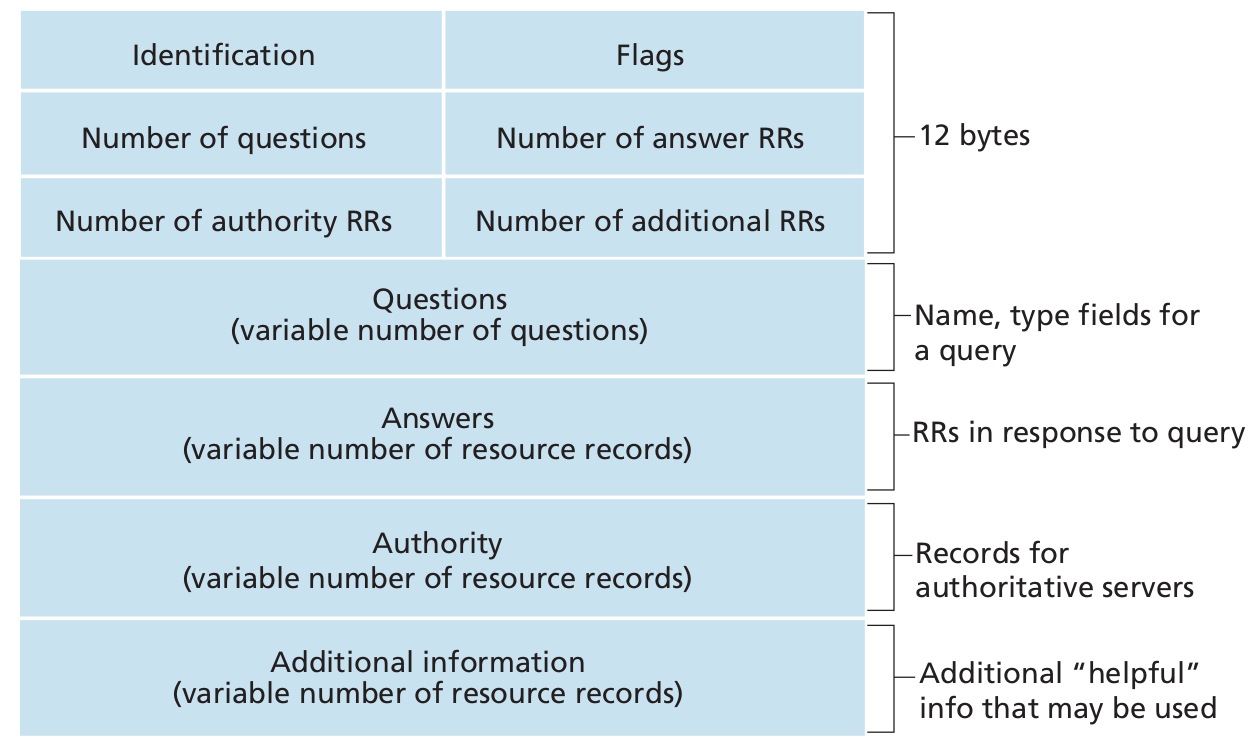
\includegraphics{img/dns_message_format.png}

  \begin{itemize}
  \tightlist
  \item
    The first 12 bytes is the header header section, which has a number
    of fields

    \begin{itemize}
    \tightlist
    \item
      The first field is a 16-bitt number that identifies the query

      \begin{itemize}
      \tightlist
      \item
        This is copied into the reply message to a query, which allows
        the client to match received replies with send queries
      \end{itemize}
    \item
      There are a number of flags in the flags field

      \begin{itemize}
      \tightlist
      \item
        A 1-bit query/reply flags indicates whether the message is a
        query (0) or a reply (1)
      \item
        A 1-bit authoritative flag is set if the DNS server is an
        authoritative server for a queried name
      \item
        A 1-bit recursion-desired flag is set when a client desires that
        the DNS server perform recursion when it doesn't have the record

        \begin{itemize}
        \tightlist
        \item
          It is set in a reply if the DNS server support recursion
        \end{itemize}
      \end{itemize}
    \item
      There are also four number fields, which indicates the number of
      occurrences of the four types of data following the header
    \end{itemize}
  \item
    The question section contains information about the query that is
    being made and it includes

    \begin{enumerate}
    \def\labelenumi{\arabic{enumi}.}
    \tightlist
    \item
      A name field that contains the name that is being query
    \item
      A type field that indicates the type of question being asked about
    \end{enumerate}
  \item
    In a reply the answer section contains the resource records for the
    name that was originally queried

    \begin{itemize}
    \tightlist
    \item
      A reply can return multiple RRs in the answer, since a hostname
      can have multiple IP addresses.
    \end{itemize}
  \item
    The authority section contains records of other authoritative
    servers
  \item
    The additional section contains other helpful records

    \begin{itemize}
    \tightlist
    \item
      For example, the answer field in a reply to an MX query contains a
      resource record providing the canonical hostname of a mail server.
    \item
      It contains a Type A record providing the IP address for the
      canonical hostname of the mail server.
    \end{itemize}
  \end{itemize}
\end{itemize}


    % Add a bibliography block to the postdoc
    
    
    
    \end{document}
